%-----------------------------------------------------------------------------
%
%               Template for sigplanconf LaTeX Class
%
% Name:         sigplanconf-template.tex
%
% Purpose:      A template for sigplanconf.cls, which is a LaTeX 2e class
%               file for SIGPLAN conference proceedings.
%
% Guide:        Refer to "Author's Guide to the ACM SIGPLAN Class,"
%               sigplanconf-guide.pdf
%
% Author:       Paul C. Anagnostopoulos
%               Windfall Software
%               978 371-2316
%               paul@windfall.com
%
% Created:      15 February 2005
%
%-----------------------------------------------------------------------------


\documentclass{sigplanconf}

% The following \documentclass options may be useful:

% preprint      Remove this option only once the paper is in final form.
% 10pt          To set in 10-point type instead of 9-point.
% 11pt          To set in 11-point type instead of 9-point.
% authoryear    To obtain author/year citation style instead of numeric.

\usepackage{amsmath}

\usepackage{color}
\usepackage{microtype}
\DisableLigatures{encoding = *, family = * }
\usepackage{graphicx}
%\usepackage{algorithm}
%\usepackage{algpseudocode}
%\renewcommand{\algorithmicrequire}{\textbf{Input:}}
%\renewcommand{\algorithmicensure}{\textbf{Output:}}
\usepackage[vlined,ruled,linesnumbered]{algorithm2e}
%\usepackage[lined,boxed,commentsnumbered]{algorithm2e}
\usepackage[pdftex]{hyperref}
\usepackage{url}

\begin{document}

\special{papersize=8.5in,11in}
\setlength{\pdfpageheight}{\paperheight}
\setlength{\pdfpagewidth}{\paperwidth}

\conferenceinfo{CONF 'yy}{Month d--d, 20yy, City, ST, Country} 
\copyrightyear{20yy} 
\copyrightdata{978-1-nnnn-nnnn-n/yy/mm} 
\doi{nnnnnnn.nnnnnnn}

% Uncomment one of the following two, if you are not going for the 
% traditional copyright transfer agreement.

%\exclusivelicense                % ACM gets exclusive license to publish, 
                                  % you retain copyright

%\permissiontopublish             % ACM gets nonexclusive license to publish
                                  % (paid open-access papers, 
                                  % short abstracts)

\titlebanner{banner above paper title}        % These are ignored unless
\preprintfooter{short description of paper}   % 'preprint' option specified.

\title{Coarse Grain Parallelization of Deep Neural Networks}
%\subtitle{Subtitle Text, if any}

\authorinfo{Blind Review}
           {}
           {}
%\authorinfo{Name2\and Name3}
%           {Affiliation2/3}
%           {Email2/3}

\maketitle

\begin{abstract}
Deep neural networks (DNN) have recently achieved extraordinary
results in domains like computer vision, speech recognition and
other. One key and essential element for this success
has been the introduction of high performance computing (HPC)
techniques within one critical step in the network deployment: the
network training. This paper describes the implementation and
analysis of a coarse grain parallelization of the DNN training algorithm
with two significant features. First, it enables multi-GPU
execution without altering the algorithm convergence rate. Second,
it exploits a parallelism level that is independent from the support
of specialized and optimized libraries. Therefore, the optimization
is immediately available for accelerating the DNN training. The parallelization
has been implemented in Caffe, a state-of-the-art DNN framework. The paper
describes the code transformations for the parallelization as well as
we identify the limiting performance factors of the approach and expose
appropriate optimizations. We show competitive performance
results for two state-of-the-art computer vision benchmarks, the
MNIST and CIFAR-10 image classifiers.

\end{abstract}

%\category{CR-number}{subcategory}{third-level}

% general terms are not compulsory anymore, 
% you may leave them out
%\terms
%term1, term2

%\keywords
%keyword1, keyword2

\newcommand{\todo}[1]{}
\renewcommand{\todo}[1]{{\color{red} TODO: {#1}}}

\section{Introduction}
Recently, deep neural networks (DNN) have achieved extraordinary 
results in domains like computer vision and speech recognition \cite{ILSVRC15, Hannun2014}. 
One key and essential element for this success
has been the introduction of high performance computing (HPC)
techniques within one critical step in the network deployment: the
network training. 
Neural networks require a training stage which typically has
very high computational demands. 
Currently, the optimization of this stage
has become the main bottleneck for a reasonable trade-off between the
final network accuracy and the actual length of the
training process \cite{JeffDean2012, Coates2013} 
% [Downpour SGD and Sandblaster L-BFGS]. 

%In most recent and successful proposals, the training stage
%takes about \todo{XXX hours} for a network with state-of-the-art 
%accuracy [REFs]. Clearly, optimizing and accelerating this process are
%key priorities in the DNN domain.

During the training process, a gradient descent algorithm minimizes a pre-defined cost function. 
Most computations
along this process correspond to basic linear algebra operations. In
general, an optimal training algorithm is built upon a very specific 
data layout mainly composed of matrices and vectors, and an iterative
procedure that invokes specialized and highly optimized basic
linear algebra subroutines (BLAS).
All the widely used DNN frameworks (e,g.: Caffe \cite{Caffe}, Theano \cite{Theano} or Torch \cite{Torch}) follow this approach. 
When it comes to optimization, 
GPU acceleration has been the most widespread adopted strategy and they have
shown extraordinary performance levels. 
GPU's are massively
parallel architectures for very fine grain parallelism and BLAS
computations make a perfect fit for them. 
But in terms of programmability,
porting the original code to GPU kernels requires significant programming 
efforts. 
The general solution has been to use specialized 
libraries like cuBLAS  \cite{cuBLAS} and cuDNN \cite{cuDNN}. 
Unfortunately, this approach lacks from generality.
During the research cycle to create a DNN, the optimal network topology,
parameters and data layout are unknown. 
So, the specialized GPU libraries are not yet useful. 
Even for the case of cuDNN, 
only DNN transformations that are very well understood 
% and no longer in a research stage 
(e.g.: convolution and pooling operations),
are supported, and has a strong bias towards computer vision applications.

An unexplored strategy is a CPU parallelization at a coarser level.
Neural networks are trained with batches of data where each batch
contains a fixed number of data samples. Each sample is used to
advance the minimization of the cost function and all samples in
the batch can be processed in parallel. This defines a much coarser
thread level parallelism but adds complexity to the
parallelization process: thread level parallelism has to be explicitly 
introduced and race conditions appear for the network coefficient 
update. 
%This has made this option not fully explored by the
%DNN community although its potential is very significant. 
The batch-level parallelism is inherent to the gradient descent 
algorithm and produces immediate acceleration irrespective of the 
nature of the network computations. It does not rely on a 
particular optimal data layout nor the availability of any specialized 
and highly optimized library for the network layers. So, its 
activation does not require 
any code porting efforts. We name this property as \textbf{network-agnostic}.
Moreover, a batch-level parallelization does not change any 
training parameter, thus it does not affect the convergence of the 
gradient descent. This is important, because parallelization strategies 
that do change the training parameters do not ensure convergence
invariance. For instance, multi-GPU systems have been explored when 
the batch and model parameters do not fit in the memory of a single GPU.
The solution has been to reduce the batch size and make it fit in memory.
But this changes the batch size and alters the convergence. In general, 
doubling the number of GPUs having halved the batch size is never a 
guarantee of observing a 2x speedup for the training 
process \cite{Hannun2014}. We name this property as \textbf{convergence-invariant}.

%would enable a multi-GPU execution
%without changing any parameter of the training algorithm. This is
%important because the convergence rate would not be affected.
%Multi-GPU systems have been explored, but only when the batch
%and model parameters do not fit in the memory of a single GPU.
%The solution has been to reduce the batch size and switch to 
%multiple GPUs. But this approach changes the batch size and thus
%alters the convergence. In general, doubling the number of GPUs
%having halved the batch size is never a guarantee of observing a
%2x speedup for the training process [Baidu deep speech].

The main contribution of this paper is the implementation and
analysis of a \textbf{network-agnostic} and \textbf{convergence-invariant} 
coarse-grain parallelization of the DNN training algorithm.
It exploits a parallelism level that is independent from the
support of specialized and optimized libraries. Therefore, the
optimization is immediately available for accelerating the DNN
training. And it is compatible with multi-GPU execution without 
altering the algorithm convergence rate. The parallelization has 
been implemented in Caffe \cite{Caffe}, a state-of-the-art DNN framework. 
The paper describes the code transformations for the parallelization 
and we also identify the limiting performance factors of the
approach and expose appropriate optimizations. We show competitive 
performance results for two state-of-the-art computer vision
datasets, MNIST \cite{MNIST,Deng2012} and CIFAR-10 \cite{CIFAR10}. 
%
In particular, in a \todo{16-core Xeon XXXX 
at XXHz we observe speedups of XXX, at similar performance levels 
of those obtained by the GPU optimized Caffe version in a NVIDIA K40 GPU.\cite{K40}}

The rest of this paper is organized as Section 2, which 
describes the main design aspects of Caffe regarding its 
parallelization. Section 3 describes the code transformations 
and optimizations for a batch-level parallelization of the 
training core of Caffe. Section 4 analyses the performance 
limiting factors of the approach and its overall performance. 
Section 5 presents the related work and finally Section 6 
concludes the paper with its main conclusions.

 

\section{The Caffe DNN Framework}
\label{sec-caffe}
Caffe is a deep learning framework for research in deep neural
networks. It is widely used across the DNN community
and has become one main platform for neural network algorithm development. 
Two main reasons justify this. Firstly, Caffe supports
many network architectures and different training algorithms for
neural networks. Secondly, Caffe is optimized with GPU acceleration.
This section describes the main operational aspects of Caffe
regarding its parallelization. 
%It is not a functional description of the framework and its capabilities for the design of neural networks. 
The main focus of this section is to describe the neural network 
training algorithm in terms of how the computations happen across 
the network, how the data flow across these layers 
and the different types and levels of parallelism that exist within each layer.

\begin{figure}[]
\centering
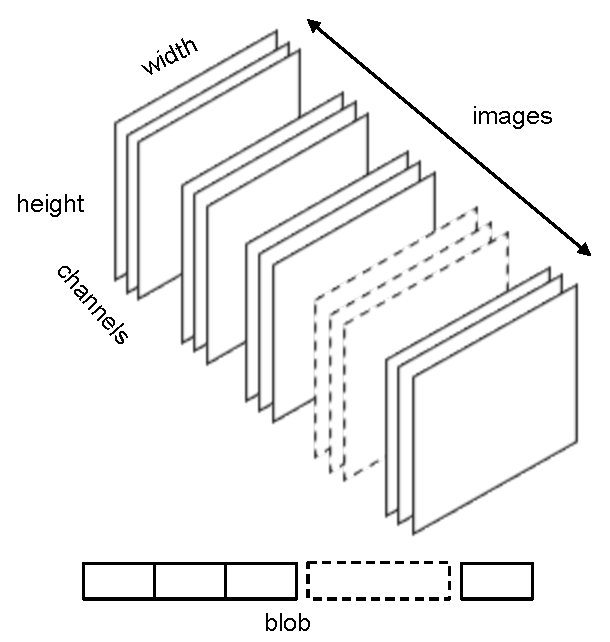
\includegraphics[width=5cm]{figures/blob1.pdf}
\caption{Example of blob structure and data segments within the blob. Each image is composed of data of three channels. Each channel is stored in one blob segment, so that every image occupies three blob segments. Images are stored sequentially one after the other within the blob.}
\label{fig-blob}
\end{figure}
\begin{figure}[]
\centering
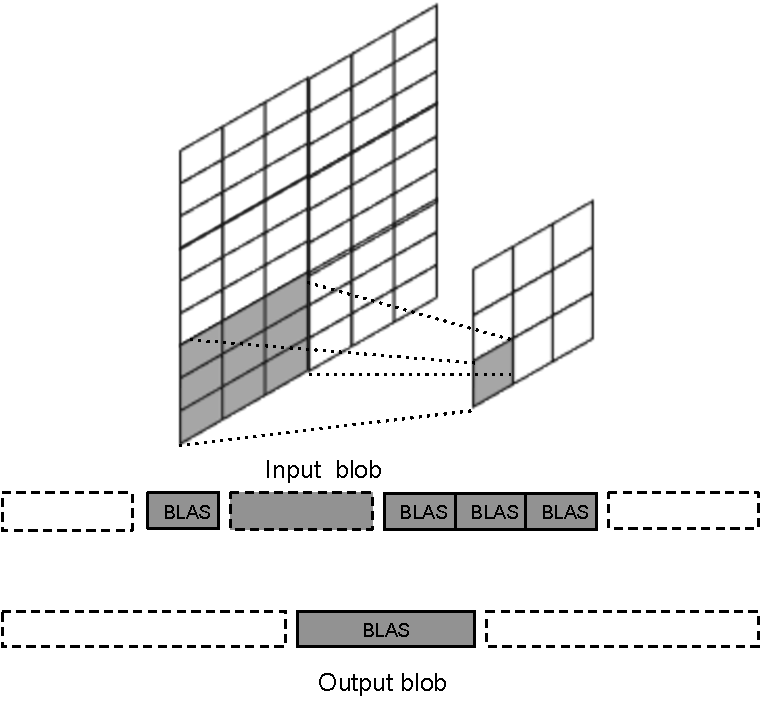
\includegraphics[width=5cm]{figures/blob2.pdf}
\caption{Example of layer transformation and its corresponding blob organization. Every 9 input segments generate the content of one segment in the output blob. This scheme is usual in deep neural networks for dimensionality reduction purposes. Pooling layers (e.g.: Caffe AVERAGE or MAX pooling layers) perform such type of computations.}
\label{fig-blob-trans}
\end{figure}

\subsection{Neural Networks in Caffe}
Caffe allows an user to specify the network structure in a prototext format \cite{protocol-buffer} 
that can capture any kind of arbitrary DAG (directed acyclic graph).
Caffe framework allows users to define their own \emph{Layers} and each layer has a pre-defined generic interface. 
Hence as users compose a network of these Layers it becomes very easily to define extremely complicated graphs in a very compact notation. 
Caffe also allows users to specify all the solver parameters as part of a \emph{Solver} file that is used for the optimization process. 
The optimization process uses back propagation and implements several algorithms such as SGD, ADAGRAD, NESTEROV. 

A network (Net) in Caffe comprises of a set of layers. In a feed-forward network each layer is stacked
such that the output of one layer becomes the input to the next immediate layer in the network graph. 
The first layer processes the input (Data) that is fed to the neural
network. Each of the subsequent layers apply a data transformation 
according to each specific layers computation. The output of Caffe is the 
set of the coefficients in each layer after the network training process is
completed. Regarding the parallelization of the training process, the
main aspects to consider are how the input/output data flow across
the network, the structure of the computation in each layer and the
training algorithm itself.

\subsubsection{Input-Output Data}
Caffe stores and communicates data using blobs. \emph{Blobs} provide a unified memory interface 
holding data; e.g., batches of images, model parameters, and derivatives for optimization.
%The data structure that implements the communication between network layers is the \emph{Blob}. 
Mathematically a Blob is an N-dimensional array stored in a C-contiguous fashion. 
Blobs also conceal the computational and overhead of mixed CPU/GPU operation by synchronizing 
from the CPU host to the GPU device as needed. 
The conventional blob dimensions for batches of image data are number N x channel K x height H x width W. 
For example, if a network is trained on image data, the input data would be organized as a 4-dimensional blob and 
the value at index (n, k, h, w) is physically located at index ((n * K + k) * H + h) * W + w within the sequential Blob data structure.
The first dimension corresponds to the image index in a batch of images and the other
three indicates the number of channels (e.g. 3 for an RGB encoded image) and the image dimensions (height and width). Figure \ref{fig-blob}
shows an example of an input blob. For this case, the blob 
stores one image with 3 data segments, one per each image channel. 
Images are sequentially stored in the blob following this pattern. 
%In respect to computation and parallelization, the blob is a sequential data structure in the form of an array of elements
%that are accessed through a base address plus an offset, given the value of several index dimensions.


\subsubsection{Layer Computation}
Each layer performs a data transformation by operating on the input blobs and generates
output blobs. 
%that is usually based on basic linear algebra operations. 
These operations are computed in a piecewise manner 
throughout the input blob. The input blob/s are organized in
data segments where the linear algebra operations are applied. The
size of the segments is constant and layer dependent. The output
of the computation are blob/s, again organized in fixed size
segments. The computation of a layer is built upon an iterative
structure that traverses the segments in the input blob/s and applies
a specific transformation based on one or more BLAS computations 
on each segment. The output of the processing of one input data 
segment is stored in one segment in the output blob. 
Figure. \ref{fig-blob-trans} shows an example for this computational 
scheme as well as the relation between the input and output blobs 
for a layer computation. Shadowed patches correspond data segments 
in the blobs. In this case, 9 data segments in the input blob are 
used to compute a one segment in the output blob. 

In general, such transformations are implemented using basic algebra 
operations like matrix-$\times$-vector or matrix-$\times$-matrix products and are often referred to as Level 2/3 BLAS operations \cite{blackford2002updated,dongarra2002preface}. 
A layer can be understood as a procedure based on several functions in the 
form of f$_i$(x, W$_i$, b$_i$) = W$_i$x + b$_i$. The layer coefficients 
would correspond to the matrices W$_i$ and vectors b$_i$. Input x would 
correspond to a data segment in the input blob. The training process 
of a neural network optimizes the W$_i$ and b$_i$ coefficients so that 
the network accuracy is maximized for a particular data model.

\subsubsection{Neural Network Training}
The training process of a neural network is based on the gradient
descent algorithm. The algorithm continuously seeks the minimization of a cost function along training epochs, where one epoch 
constitutes of processing all the training data samples. These are 
grouped in batches of fixed size and during every epoch each batch 
is processed in two steps. First, the batch samples are used to 
compute the average error of the network. The samples 
traverse the network where each layer applies its transformation and 
temporally stores its output in a blob. This phase is identified as 
the \emph{forward pass} of the network. Second, the network computes the 
gradient of its transformation as a whole. In this phase, every layer 
applies the chain rule for propagating the derivatives across the layers in the backward direction. From the 
last layer up to the first one in the network, each layer propagates 
its output multiplied by its derivative value. This phase is identified 
as the \emph{backward pass}. Both the forward and backward pass are 
inherently sequential as both the output and the gradients have to 
be propagated through the layers in an upward and downward manner across 
the network. Algorithms \ref{alg-train}, \ref{alg-forw} and \ref{alg-back} 
show the high level structure of the training algorithm as well as 
how the data flow across the layers in the forward and backward pass.
 
%\IncMargin{1em}
\begin{algorithm}
\small
\caption{Iteration of the DNN training algorithm.}
\label{alg-train}
%\SetKwData{Left}{left}\SetKwData{This}{this}\SetKwData{Up}{up}
%\SetKwFunction{Union}{Union}\SetKwFunction{FindCompress}{FindCompress}
\SetKwInOut{Input}{input}\SetKwInOut{Output}{output}
%\KwData{batches}
%\KwResult{batches}
\Input{B, batches}
\Output{Network layer coefficients}
\BlankLine
%\Begin{
%\While{loss not acceptable}{
\For{$b\leftarrow 1$ \KwTo $B$}{
%  \For{$s\leftarrow 1$ \KwTo $S$}{
\BlankLine
    top[1]=layers(1)$\rightarrow$ forward(batches[b]);
\BlankLine
    \For{$l\leftarrow 2$ \KwTo $L$}{
      top[l]=layers(l)$\rightarrow$ forward(top[l-1]);
    }
\BlankLine
    diffs[1]=layers(L)$\rightarrow$ backward(top[L]);
\BlankLine
    \For{$l\leftarrow L-1$ \KwTo $1$}{
      diffs[l]=layers(l)$\rightarrow$ backward(top[l],diffs[l+1]);
    }
updateCoefficients(layers, top, diffs);
  }
%}
%loss = evaluateNetwork(layers);
%}
%}
\end{algorithm}
%\DecMargin{1em}

Algorithm \ref{alg-train} corresponds to one training iteration. 
Each data batch \emph{b} is propagated through the network. 
First layer processes the batch and outputs the first transformation 
for each sample in it. This is than forwarded to the 
second layer to apply the next transformation. This process continues 
until all layers have applied their transformation. The last layer 
of the network is the one responsible to check the output of the 
network and evaluate the network accuracy. The loop in line 3 implements 
the batch network computation, the network forward phase.
This loop is inherently sequential and each layer 
transformation happens within the \emph{forward} call. The output of 
this call is stored in vector \emph{top} for all data samples in the 
batch. Each \emph{forward} invocation uses as input the \emph{top} 
produced by the previous layer. Loop in line 6 corresponds to the 
computation of network gradients. Once the network has been evaluated 
with one batch, the algorithm computes every layers gradient 
with respect its input. This process seeks the minimization 
of the network error. This loop is also inherently sequential and 
the \emph{backward} call computes the layer gradient, \emph{diffs}. 
This process requires both the evaluation of the layer transformation 
(\emph{top}) and the previous gradient computed in the immediate previous 
layer (\emph{diffs}) in backward manner. It corresponds to the network 
backward phase. Once both the forward and backward phases are completed, 
the training algorithm updates the network coefficients in all layers. 
This corresponds to line 8 and procedure call to \emph{updateCoefficients}.

\begin{algorithm}
\small
\caption{Layer forward phase}
\label{alg-forw}
%\SetKwData{Left}{left}\SetKwData{This}{this}\SetKwData{Up}{up}
%\SetKwFunction{Union}{Union}\SetKwFunction{FindCompress}{FindCompress}
\SetKwInOut{Input}{input}\SetKwInOut{Output}{output}
\Input{Bottom blob (S, N+1, $D_1, D_2$, $\dots$, $D_N$)}
\Output{Top blob for the layer transformation}
\BlankLine
\For{$s \leftarrow 1$ \KwTo $S$}{
\BlankLine
\For{$d_1 \leftarrow 1$ \KwTo $D_1$}{
  \For{$d_2 \leftarrow 1$ \KwTo $D_2$}{
    \dots 
\BlankLine
    \For{$d_N \leftarrow 1$ \KwTo $D_N$}{
      top[f(s, $d_1,d_2$, $\dots$, $d_N$)]=\textbf{BLAS}(W($d_1,d_2$, $\dots$, $d_N$), b($d_1,d_2$, $\dots$, $d_N$), bottom[g(s, $d_1,d_2$, $\dots$, $d_N$)]);
}
}
}
}
\end{algorithm}

\begin{algorithm}
\small
\caption{Layer backward phase}
\label{alg-back}
%\SetKwData{Left}{left}\SetKwData{This}{this}\SetKwData{Up}{up}
%\SetKwFunction{Union}{Union}\SetKwFunction{FindCompress}{FindCompress}
\SetKwInOut{Input}{input}\SetKwInOut{Output}{output}
\Input{Gradient w.r.t. top blob (S, N+1, $D_1, D_2$, $\dots$, $D_N$)}
\Output{Gradient w.r.t. to bottom blob}
\BlankLine
\For{$s \leftarrow 1$ \KwTo $S$}{
\BlankLine
\For{$d_1 \leftarrow 1$ \KwTo $D_1$}{
  \For{$d_2 \leftarrow 1$ \KwTo $D_2$}{
\BlankLine
    \dots 
\BlankLine
    \For{$d_N \leftarrow 1$ \KwTo $D_N$}{
      diffs\_bottom[f(s, $d_1,d_2$, $\dots$, $d_N$)]=\textbf{BLAS}(W($d_1,d_2$, $\dots$, $d_N$), b($d_1,d_2$, $\dots$, $d_N$), top[h(s, $d_1,d_2$, $\dots$, $d_N$)], diffs\_top[g(s, $d_1,d_2$, $\dots$, $d_N$)]);
}
}
}
}
\end{algorithm}

Algorithm \ref{alg-forw} corresponds to the description of the structure 
of one layer transformation. In general, the layer computation is organized 
in a nest of loops that traverse the \emph{N+1} dimensions (\emph{S, D$_1$, 
D$_2$, \dots, D$_N$}) of the layer input blob \emph{bottom} and produces 
a transformation stored in the output blob \emph{top}. The first dimension 
corresponds to the data samples in the batch. These are indexed with the 
variable \emph{s}.  According to layer specific functions 
(\emph{f} and \emph{g} in line 5 of the algorithm), 
data segments in the input/ouput blobs are processed through basic linear 
algebra transformations (\emph{BLAS} call in line 5) that are also 
dependent to the data segment being processed (\emph{W} and \emph{b} 
depend on the loop induction variables). Algorithm 
\ref{alg-back} follows a very similar structure, but operating with 
blobs that store the gradient computation (\emph{diffs\_bottom} and 
\emph{diffs\_top}).


%\begin{figure*}[]
%\centering
%%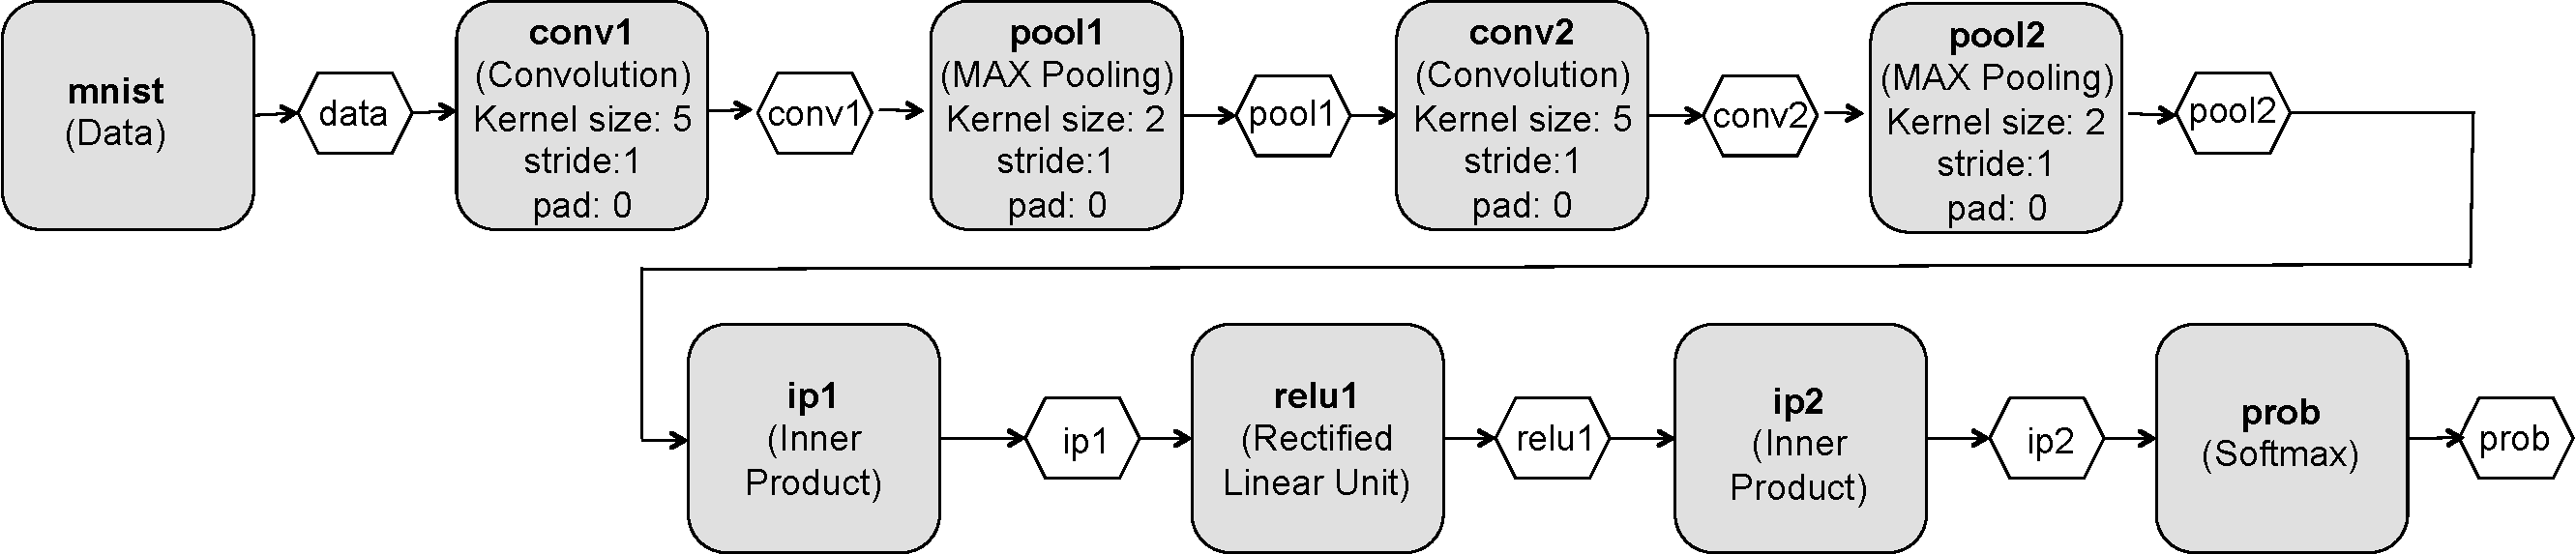
\includegraphics[width=\textwidth]{figures/mnist.pdf}
%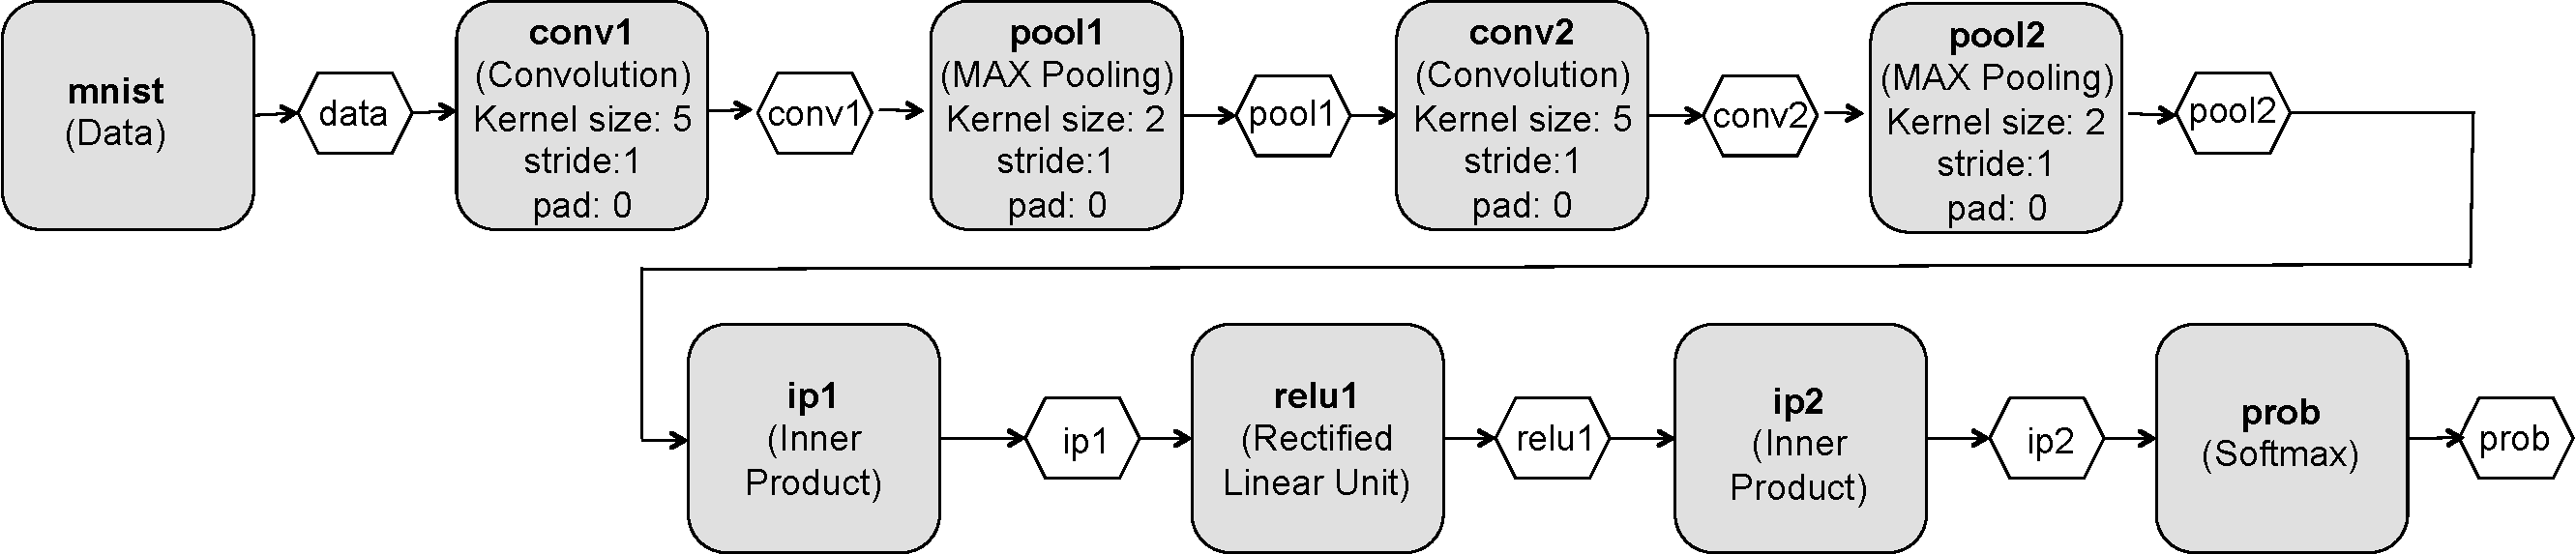
\includegraphics[height=2cm]{figures/mnist.pdf}
%%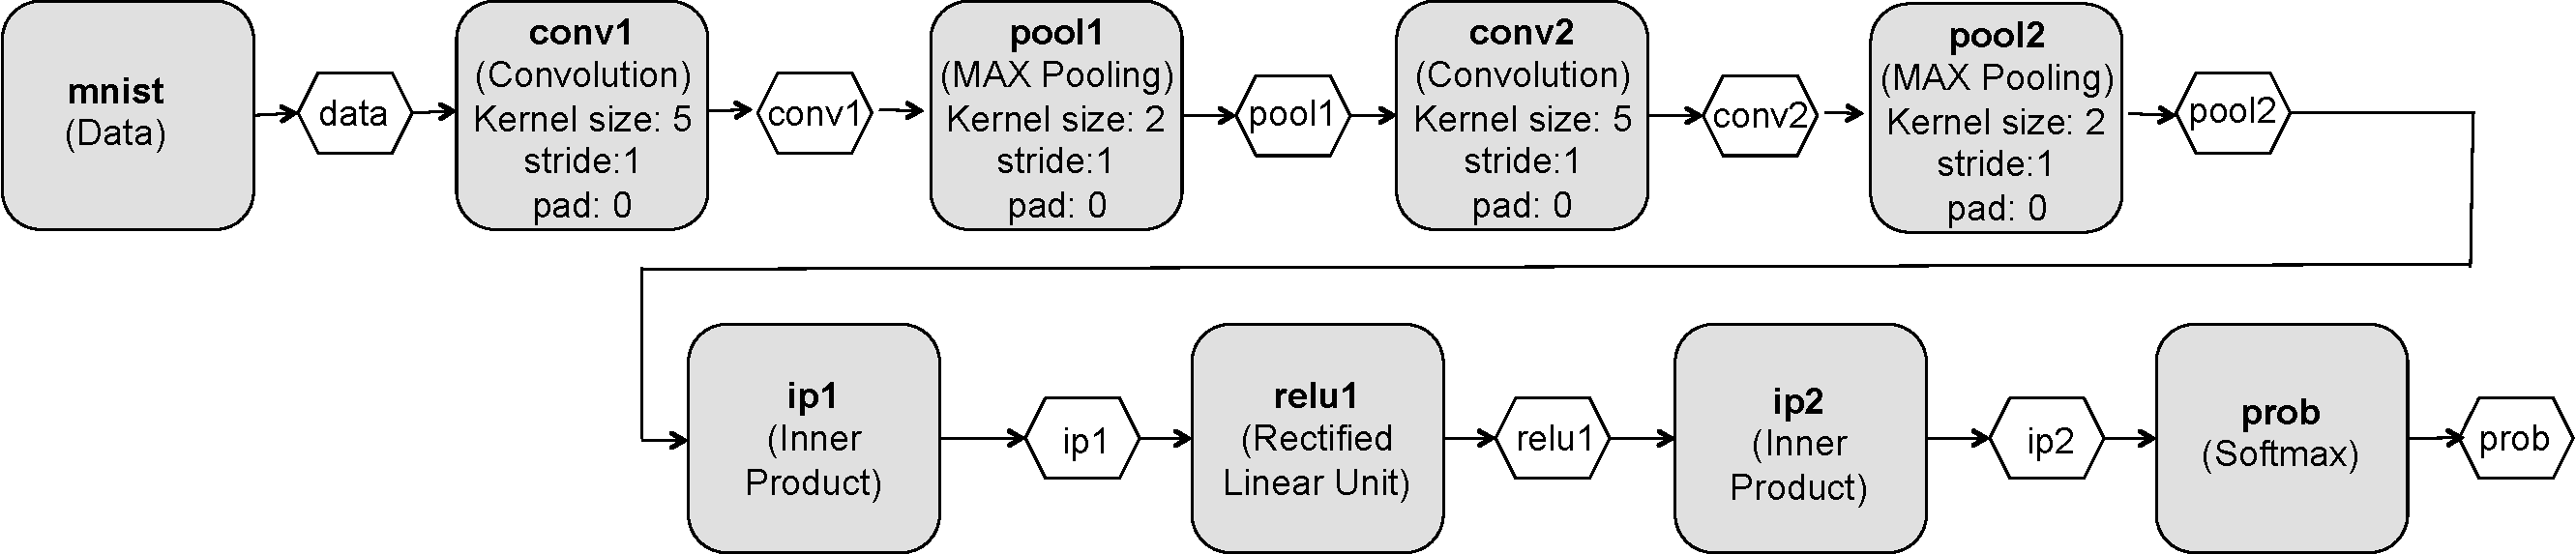
\includegraphics[width=13.5cm]{figures/mnist.pdf}
%\caption{MNIST network: composed of 9 layers, organized in two sections. First data plus convolutional and pooling layers. Second, inner product and rectified linear units and loss.}
%\label{fig-mnist}
%\end{figure*}
%
%\begin{figure*}[]
%\centering
%%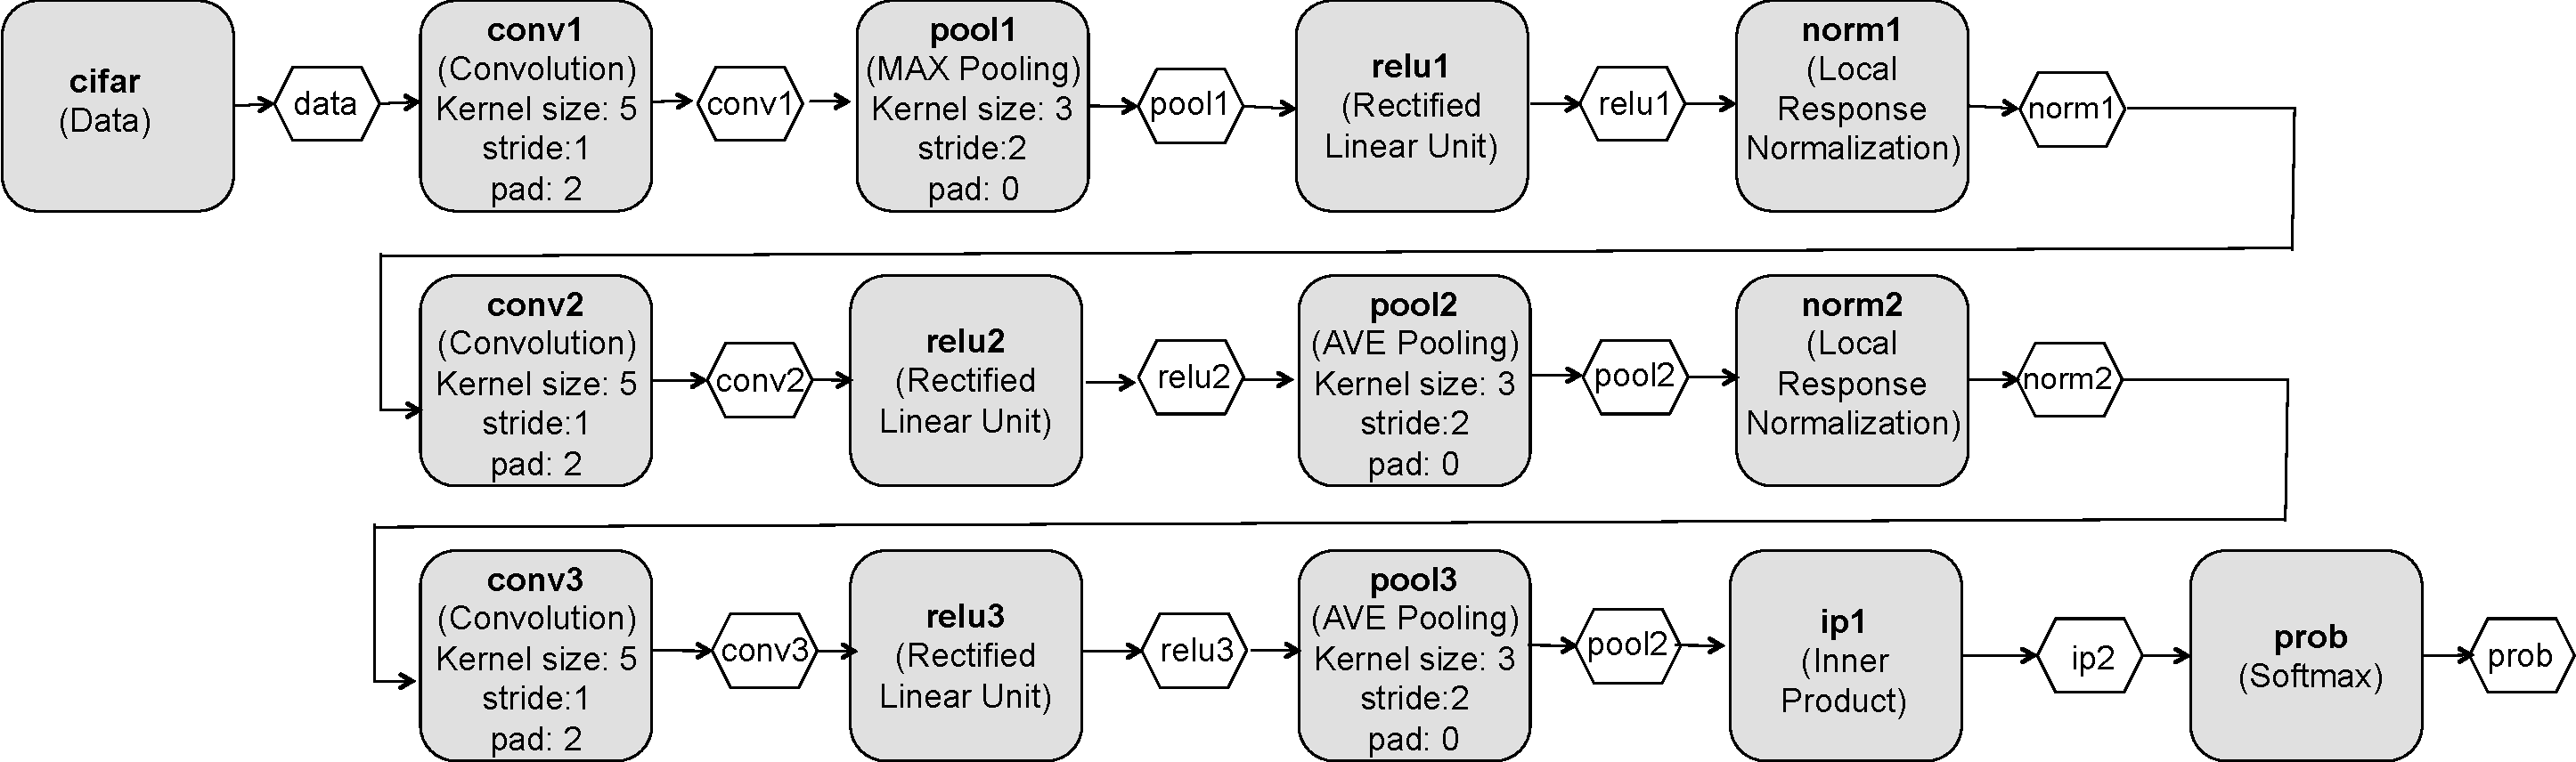
\includegraphics[width=\textwidth]{figures/cifar.pdf}
%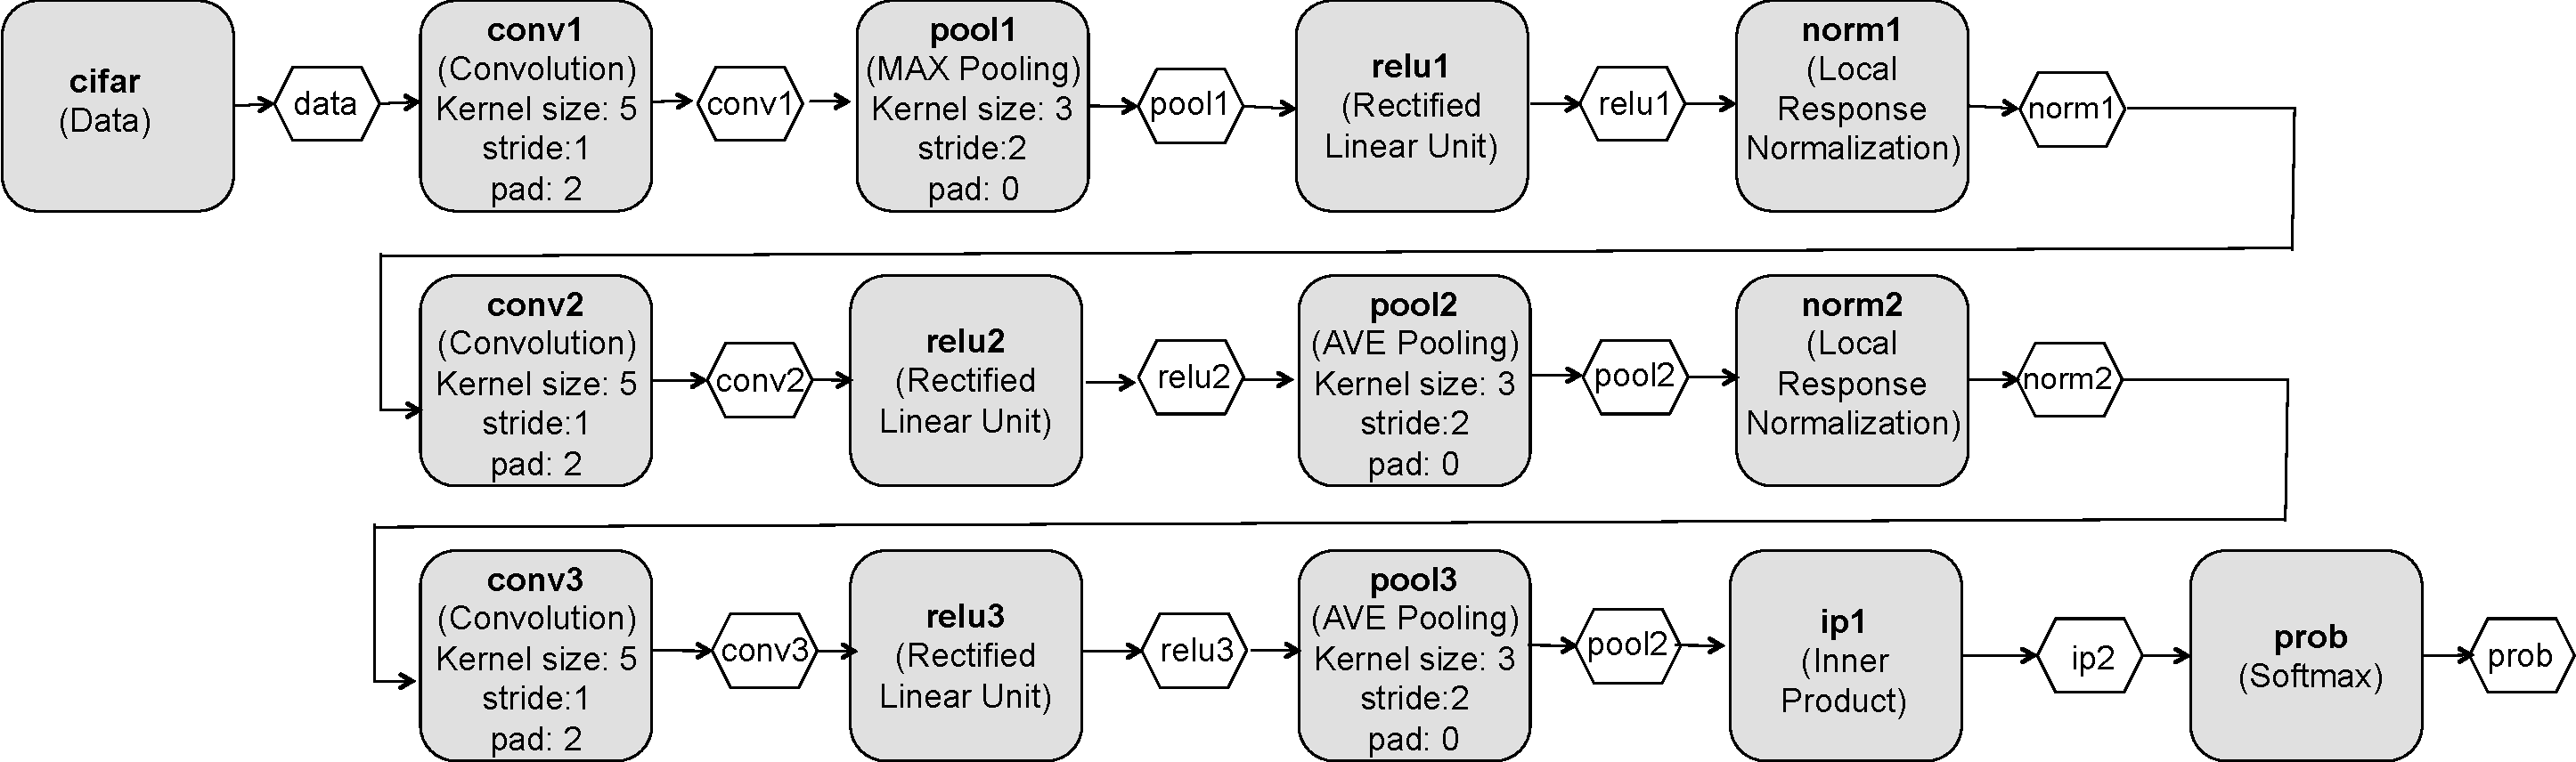
\includegraphics[height=3.5cm]{figures/cifar.pdf}
%%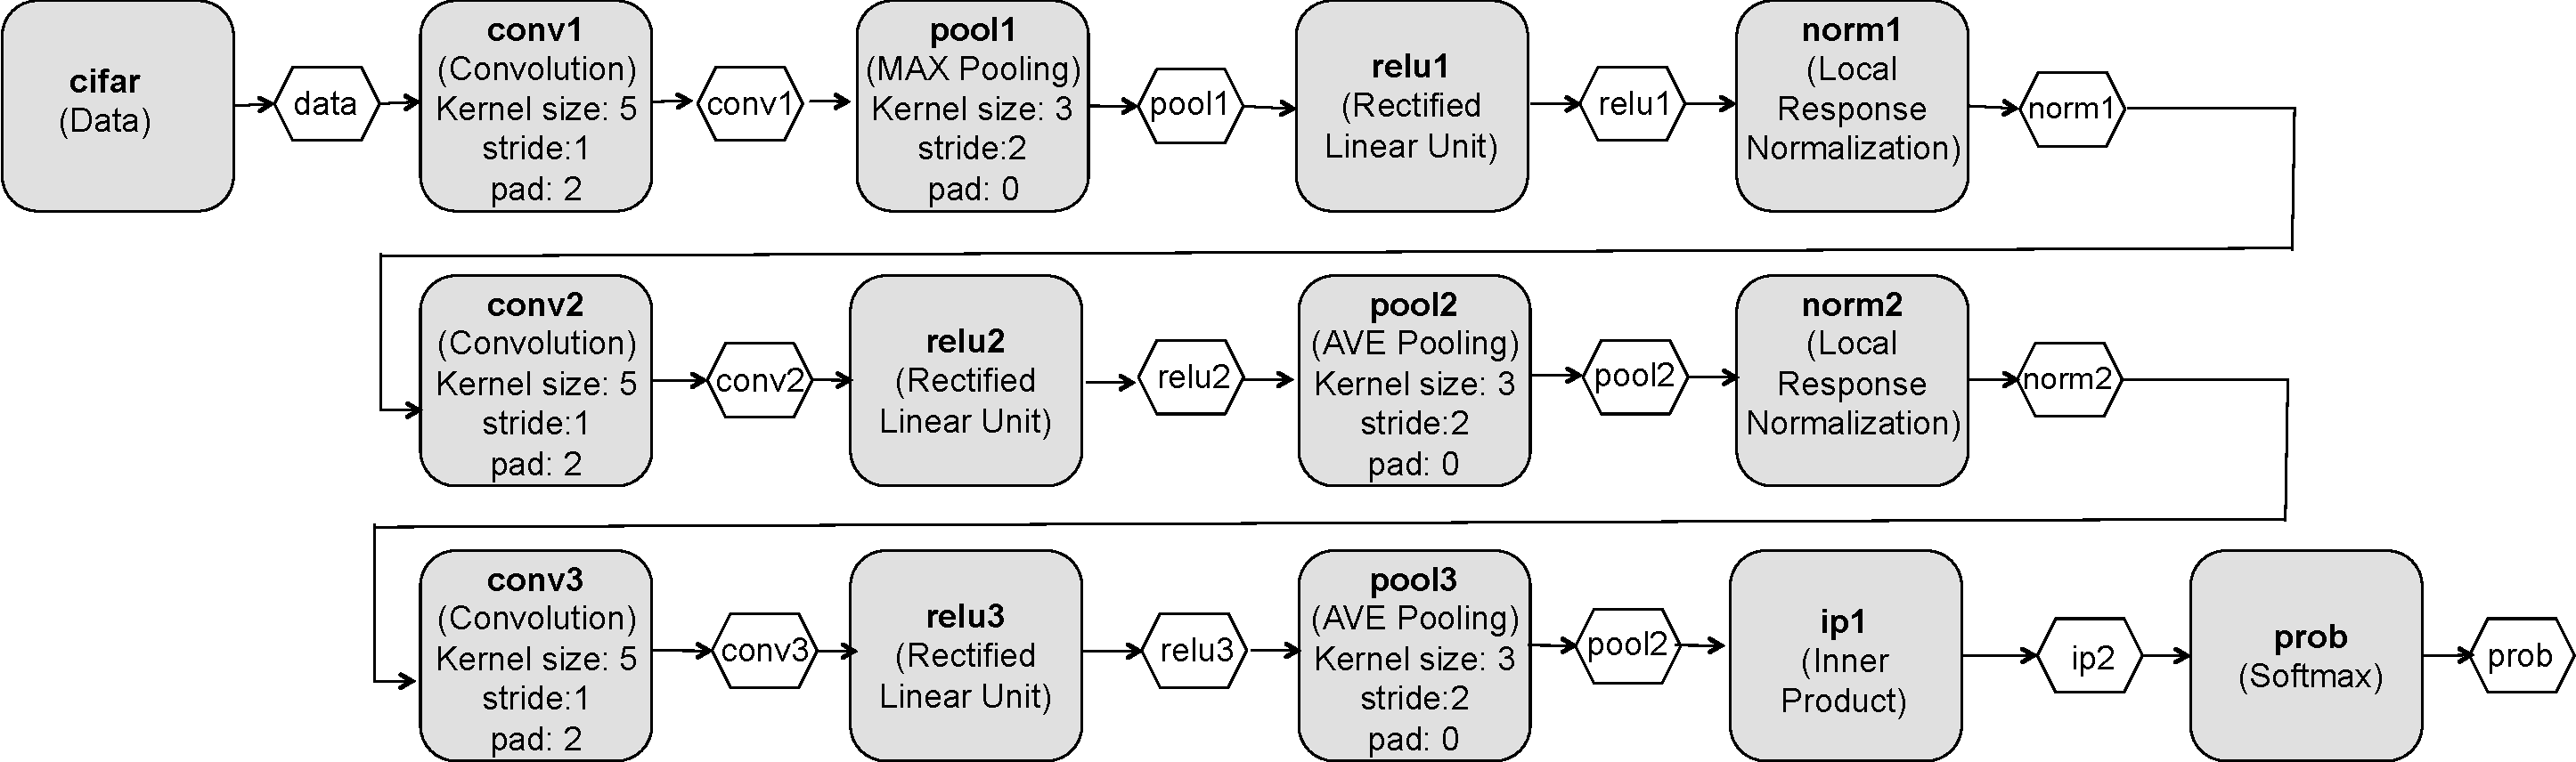
\includegraphics[width=15cm]{figures/cifar.pdf}
%\caption{CIFAR-10 network: composed 14 layers, organized in two sections. First, data plus convolutional, pooling, rectified linear units and local response normalization layers. Second, pooling and inner product and loss.}
%\label{fig-cifar}
%\end{figure*}

\begin{figure*}[]
\centering
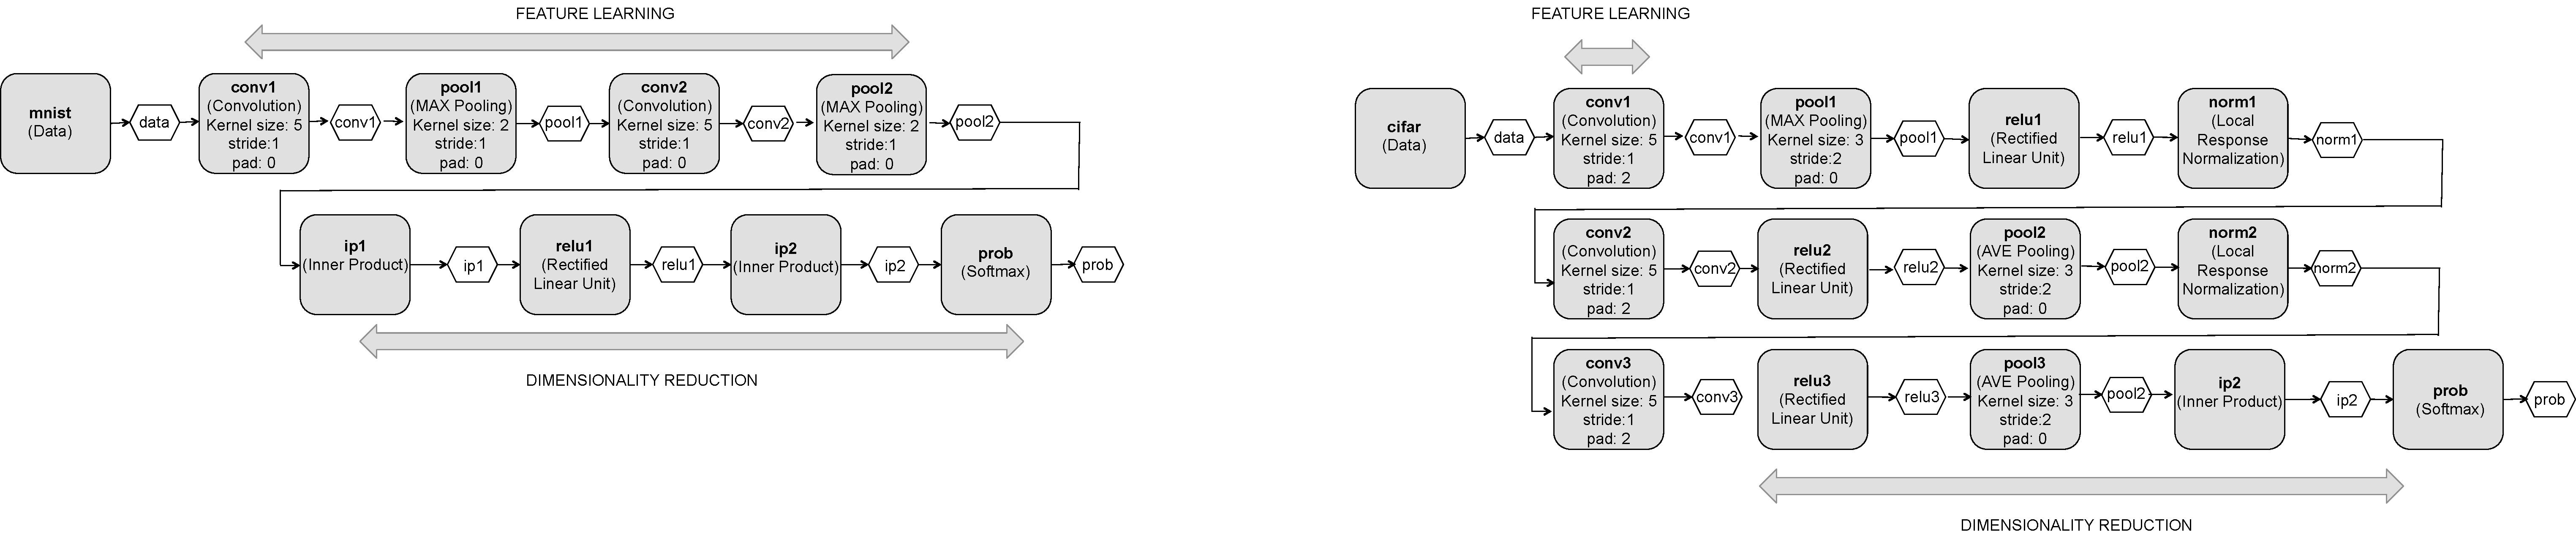
\includegraphics[width=\linewidth]{figures/mnist-cifar.pdf}
\caption{MNIST network: composed of 9 layers, organized in two sections. First data plus convolutional and pooling layers. Second, inner product and rectified linear units and loss. CIFAR network: composed 14 layers, organized in two sections. First, data plus convolutional, pooling, rectified linear units and local response normalization layers. Second, pooling and inner product and loss.}
\label{fig-mnist-cifar}
\end{figure*}

\subsection{Network Examples: MNIST and CIFAR-10}
The MNIST \cite{Deng2012, MNIST} and CIFAR-10 \cite{CIFAR10} datasets are standard datasets for 
computer vision. The MNIST dataset is composed of 60,000 images, each of dimension 28$\times$28 pixels 
of handwritten digits for training and 10,000 test examples. 
The Caffe distribution includes the LeNet \cite{LeNet} network for generating an image 
classifier for this dataset. Given an a handwritten digit, 
the network outputs which digit is represented (e.g.: 0 \dots 9). 
The CIFAR-10 is a CNN (Convolution Neural network) \cite{CNN} included in the Caffe distribution
that performs as an image classifier for the CIFAR dataset. CIFAR is 
composed of 60,000 32$\times$32 color images with 10 classes: 
\emph{airplane, automobile, bird, cat, deer, dog, frog, horse, ship, 
truck} with 6000 images per class. Both the networks are built with  
a subset of the available layers within Caffe. 

\subsubsection{Types of Layers}
Caffe supports a great variety of network layers. The following 
paragraph describes the layers that are mostly used for computer vision, and 
in particular, for the two example networks studied in this paper.
The \textbf{Data Layer} corresponds to the first layer in the 
network. This layer is responsible of fetching the data in batches and 
feeding it to the network. The \textbf{Convolutional Layer} applies 
a group of convolutions to an image. Its parameters are the size of the 
convolutional patch and the stride to apply along the image, among others. 
In general, the coefficients in this type of layer are learnt so that 
they capture what are the relevant data features 
for the image classification. The \textbf{Pooling Layer} usually 
follows the convolutional layer. In general, this layer applies an averaging 
function over a subset of data points. The most usual functions are the 
MAX pooling function, when the pooling layer selects the maximum value for the 
subset, and the AVERAGE function, when the pooling layer computes the average 
value of the subset. The \textbf{Local Response Normalization Layer} 
performs a local normalization over a local region in the image. 
This normalization can happen across the image channels or within the image 
channels. The \textbf{Rectified Linear Unit Layer (ReLU)} computes 
the max(x,0) function for each element in its input blob. 
The \textbf{Inner Product Layer} also identified as a fully-connected layer, 
performs a vector product between its input and coefficients.  
The \textbf{Loss and Accuracy Layers} correspond 
to the deepest layers in the network. They are responsible for evaluating the 
loss function for the gradient computation and the overall network accuracy.

\subsubsection{Networks}
The aim of this section is to briefly introduce the two networks 
used in this paper. The section describes the network layers and characterizes 
them in terms of feature learning layers and dimensionality reduction 
layers. Regarding the parallelization, it is important to notice that 
the deeper the layers, the smaller the size of the input/output blobs. 
Thus, the level in the network will affect the work granularity of the 
existing parallelism within the layer. 

Figure \ref{fig-mnist-cifar} shows the layer composition for the MNIST network. 
This network is composed of an initial data layer followed by the 
combination of two instances of convolutional and pooling layers. The 
convolutional layers are responsible for feature learning while the 
pooling layers correspond to dimensionality reduction. 
This is followed by a inner product layer (ip) and ReLU layer which furthermore reduces the dimensionality 
of the data traversing the network, until the last inner product layer which 
outputs a vector of 10 elements, one per digit class. The last layer 
corresponds to a loss layer.  
Figure \ref{fig-mnist-cifar} shows the layer composition for the CIFAR network. 
As in the previous network, the first layer is a data layer, followed by 
the combination of convolutional, ReLU and pooling layers. Again, convolutional 
layers perform the feature learning and pooling layers perform the 
dimensionality reduction. The ReLU layer controls the saturation of 
the output of the convolutional coefficients. CIFAR also includes 
normalization layers between the first two instances of convolution and pooling 
layers.  The inner product layer (ip) and loss layer (SoftMax) are the last layers of the network. 

 

\section{Caffe Coarse Grain Parallelization}
This section describes the parallelization process for a coarse-grain 
parallelization in the Caffe DNN framework. First, we identify the 
different sources of parallelism and their granularity. Second, we 
describe the methodology to generate a coarse-grain parallelism version 
of the algorithms discussed previously in section \ref{sec-caffe}. Finally, 
we compare our approach to that of a fine-grain parallelization 
corresponding to the GPU version.

\subsection{Sources of Parallelism}
Given the structure of the computation in algorithms \ref{alg-train}, 
\ref{alg-forw} and \ref{alg-back}, the training procedure of a neural 
network exposes several levels and types of parallelism.

\subsubsection{BLAS Level Parallelism}
This level of parallelism corresponds to the computations that 
are based on basic linear algebra operations. It appears in the 
BLAS computations executed for each data segment in the input/output blobs.
In algorithms \ref{alg-forw} and \ref{alg-back} the BLAS calls in line 
6 in both cases hide this level of parallelism.
In general, these computations correspond to matrix and
vector operations like matrix-$\times$-vector and matrix-$\times$-matrix
products. Caffe includes a native and limited BLAS implementation that 
can be substituted with specialized libraries like Atlas, OpenBLAS  or Intel MKL \cite{blackford2002updated,dongarra2002preface}. These implementations are highly optimized and exploit both thread level parallelism and SIMD level parallelism with vectorized code.

\subsubsection{Blob Level Parallelism}
This level of parallelism corresponds to the nested loops in the forward
and backward phases in lines 2 and 5 in algorithms 
\ref{alg-forw} and \ref{alg-back}. 
These loops traverse the data segments in the input and output blobs and
perform BLAS calls for each segment. This kind of parallelism can be
achieved with thread level parallelism as each BLAS call can be
executed in parallel.
In general, the dimensions of the input blob are layer dependent. Therefore the number of iterations in each loop level is also layer dependent. All loops are 
interchangeable and parallel, given the appropriate data privatizations. 
So, in order to have control of the most appropriate loop scheduling, 
loops can be rearranged in different manners. 

\subsubsection{Batch Level Parallelism}
This level corresponds to the loop in line 1 of algorithms \ref{alg-forw}
and \ref{alg-back}. 
This loop traverses the data samples in the batch and its parallelism 
can be exploited but with limitations. 
Specifically for the backward phase, it requires reduction operations 
for the network coefficient update. The training algorithm averages all 
gradients computed with each sample in the batch. This averaging
has to be protected with mutual exclusion operations or ordered
loops plus data privatization for the blobs that temporally store the
gradients. 


%\begin{algorithm}
%\caption{Caffe layer forward phase}
%\label{batch-forw-algo}
%%\SetKwData{Left}{left}\SetKwData{This}{this}\SetKwData{Up}{up}
%%\SetKwFunction{Union}{Union}\SetKwFunction{FindCompress}{FindCompress}
%\SetKwInOut{Input}{input}\SetKwInOut{Output}{output}
%\Input{Bottom blob (N, $D_1, D_2$, $\dots$, $D_N$)}
%\Output{Top blob for the layer transformation}
%\BlankLine
%\For{$s \leftarrow 1$ \KwTo $S$}{
%\For{$d_1 \leftarrow 1$ \KwTo $D_1$}{
  %\For{$d_2 \leftarrow 1$ \KwTo $D_2$}{
%\BlankLine
    %\dots
%\BlankLine
    %\For{$d_N \leftarrow 1$ \KwTo $D_N$}{
      %top[f($d_1,d_2$, $\dots$, $d_N$)]=\textbf{BLAS}(W, bias, bottom[g($d_1,d_2$, $\dots$, $d_N$)]);
%}
%}
%}
%}
%\end{algorithm}

\begin{algorithm}
\setstretch{0.25}
\small
%\algsetup{linenosize=\footnotesize}
\caption{Coarse-grain parallel layer forward phase}
\label{alg-par-forw}
%\SetKwData{Left}{left}\SetKwData{This}{this}\SetKwData{Up}{up}
%\SetKwFunction{Union}{Union}\SetKwFunction{FindCompress}{FindCompress}
\SetKwInOut{Input}{input}\SetKwInOut{Output}{output}
\Input{Bottom blob (S, N+1, $D_1, D_2$, $\dots$, $D_N$)}
\Output{Top blob for the layer transformation}
%\BlankLine
%\#pragma omp parallel for 
\textbf{\#pragma omp parallel}
%\BlankLine
\{
\BlankLine
\emph{/* Object Privatization */}
%\BlankLine
\dots
\BlankLine
\textbf{\#pragma omp for private($s$, $d_1$, $d_2$, \dots)}
\BlankLine
\For{$civ \leftarrow 1$ \KwTo $S*D_1$$*D_2$*$\dots$*$D_k$}{
    %\BlankLine
    s = $f_s$(civ);
    \BlankLine
    $d_1$ = $f_1$(civ);
    \BlankLine
    $d_2$ = $f_2$(civ);
    \BlankLine
    \dots
    \BlankLine
    $d_k$ = $f_k$(civ);
    \BlankLine
    \For{$d_{\text{k+1}}$ $\leftarrow 1$ \KwTo $D_{\text{k+1}}$}{
    \BlankLine
    \dots
    \BlankLine
    \For{$d_N \leftarrow 1$ \KwTo $D_N$}{
      top[f(s, $d_1,d_2$, $\dots$, $d_N$)]=\textbf{BLAS}($W$($d_1,d_2$, $\dots$, $d_N$), bias($d_1,d_2$, $\dots$, $d_N$), bottom[g(s, $d_1,d_2$, $\dots$, $d_N$)]);
}
}
}
\}
\end{algorithm}

\subsection{Code Transformations}
The Caffe framework is designed using object-oriented methodologies and uses a C++ implementation. 
Its main data structures and algorithms have been designed with 
functional principles with the aim of giving support for neural network 
development. In this paper, we have followed a methodology to 
parallelize Caffe so that these principles are kept intact. We wanted to minimize 
code reorganization for the optimization process.
To indicate the parallelism to be exploited, only directive-based 
transformations have been applied. We have used OpenMP \cite{basumallik2007programming} directives 
to indicate which loops have to be parallelized. Whenever possible, 
we have used the OpenMP primitives to indicate data privatizations 
and reduction operations, as well as the necessary synchronization 
points along the parallel code. To increase performance, we have 
applied very simple manual code transformations like loop coalescing or 
loop interchange. Therefore, in order to enable a coarse-grain 
parallelization, no object data structure has been modified and 
the implementation of every Caffe layer has not been recoded with 
any platform-specific optimization.

\subsubsection{Coarse grain parallelization and optimizations}
Algorithm \ref{alg-par-forw} shows a high level description of a 
coarse grain parallelization of the forward layer transformation 
described in section \ref{sec-caffe}. The parallelization is specified 
with directive-based annotations following the OpenMP syntax and semantics. 
Coarse parallelism is defined by a parallel region that englobes all the 
layer code (lines 1-16). The original loop nest appears with a coalescing 
transformation where some of the outermost loops have been collapsed into a 
single loop statement (line 6). A parallelizing directive for this loop 
is inserted (line 5) specifying the parallel execution of this loop 
under a static loop scheduling (default scheduling for OpenMP \cite{basumallik2007programming}). 
The loop coalescing transformation is related to the parallelization 
process and is done to have effective control of the work distribution 
under a static loop scheduling. To understand this issue, recall the 
code structure in Algorithm \ref{alg-forw}. In that version, the outermost 
loop corresponds to the loop that processes every data sample in the 
batch (loop with variable \emph{s}). In general, after the 
parallelization under a static scheduling, one iteration is the minimal 
work unit for work distribution. If that loop were parallelized, the 
amount of work per iteration is coarse enough so that any difference 
in the number of assigned iterations per thread can cause a significant  
work unbalance. To maintain the coarse level parallelization, but minimize 
the size of the work unit, the coalescing transformation increments the 
total number of iterations, but having every iteration a smaller 
amount of work. In general, the number of coalesced loops is layer 
dependent. Some of the layers are parallelized with no coalescing, 
other coalesce the whole loop nest. This optimization process was 
manually performed.

Algorithm \ref{alg-par-back} shows the coarse-grain parallelization of 
the backward layer pass. For parallelism specification and work 
distribution, the transformations are the same as in the previous 
case for the layer forward pass. The same coalescing transformation has 
been applied and parallelism has been specified at the same levels. 
The number of coalesced loops is layer dependent, and this optimization 
has been manually performed. The main difference resides on the special 
treatment for the gradient update (\emph{diffs\_top} and \emph{diffs\_bottom} 
variables). Recall that the DNN training algorithm averages all gradients 
computed within a batch. This happens during the layer backward phase.
Now, this computation has been parallelized, so the gradient update has 
to be implemented through a reduction operation and thread mutual exclusion 
mechanisms. In the algorithm, this corresponds to lines 18-20. An ordered loop 
is added so that every thread incorporates its gradient computation to 
the global variable that stores the gradients.
This mechanism requires the per-thread privatization of the blob storing 
the gradients. The private storage for the gradients has to be properly 
initialized to the neutral value of the reduction operation, in the case 
the zero value (lines 4-5 in the algorithm). 

\begin{algorithm}
\setstretch{0.15}
\small
\caption{Coarse-grain parallel layer backward phase}
\label{alg-par-back}
%\SetKwData{Left}{left}\SetKwData{This}{this}\SetKwData{Up}{up}
%\SetKwFunction{Union}{Union}\SetKwFunction{FindCompress}{FindCompress}
\SetKwInOut{Input}{input}\SetKwInOut{Output}{output}
\Input{Gradient w.r.t. top blob (S, N+1, $D_1, D_2$, $\dots$, $D_N$)}
\Output{Gradient w.r.t. to bottom blob (M, $O_1, O_2$, $\dots$, $O_M$)}
\BlankLine
%\#pragma omp parallel for 
\textbf{\#pragma omp parallel}
\BlankLine
\{
\BlankLine
\emph{/* Object Privatization */}
\BlankLine
Blob private-diffs-bottom(M, $O_1, O_2$, $\dots$, $O_M$);
\BlankLine
caffe\_zero($S*O_1$$*O_2$*$\dots$*$O_M$, private-diffs\_bottom);
\BlankLine
\dots
\BlankLine
\textbf{\#pragma omp for private($s$, $d_1$, $d_2$, \dots)}
\BlankLine
\For{$civ \leftarrow 1$ \KwTo $S*D_1$$*D_2$*$\dots$*$D_k$}{
    \BlankLine
    s = $f_s$(civ);
    \BlankLine
    $d_1$ = $f_1$(civ);
    \BlankLine
    $d_2$ = $f_2$(civ);
    \BlankLine
    \dots
    \BlankLine
    $d_k$ = $f_k$(civ);
    \BlankLine
    \For{$d_{\text{k+1}}$ $\leftarrow 1$ \KwTo $D_{\text{k+1}}$}{
    \BlankLine
    \dots
    \BlankLine
    \For{$d_N \leftarrow 1$ \KwTo $D_N$}{
      private-diffs-bottom[f(s, $d_1,d_2$, $\dots$, $d_N$)]=\textbf{BLAS}($W$($d_1,d_2$, $\dots$, $d_N$), bias($d_1,d_2$, $\dots$, $d_N$), top[h(s, $d_1,d_2$, $\dots$, $d_N$)], diffs-top[g(s, $d_1,d_2$, $\dots$, $d_N$)]);
}
}
}
\textbf{\#pragma omp for ordered}
\BlankLine
\For{$th \leftarrow 1$ \KwTo $omp\_get\_num\_threads()$}{
  caffe\_add(diffs-bottom, private-diffs-bottom, \dots);
}
\}
\end{algorithm}
\subsection{Coarse-grain vs Fine-grain parallelization}
The aim of this section is to describe the main differences between 
the coarse-grain and fine-grain approaches when it comes to the 
parallelization of a layer transformation. If for the coarse-grain 
case the outermost loop is parallelized after approapriate loop 
coalescing, the fine-grain approach focusses on the innermost loops.
Similarly, this approach coalesces as much as possible inner loops 
so that enough work is generated for the fine-grain threads in 
the GPU device. It is this process what requieres consideable programming 
efforts. The inner loop coalescing has to be done having in mind the 
work distribution mechanisms for GPU threads. Here we refer to the 
thread \emph{blocks} and \emph{grids}. In general, the more loops 
are coalesced, the more effective the parallelization. Regarding the 
programming efforts, after the loop transformation, the resulting loop 
has to be extracted and generate a GPU kernel. Also, introduce all 
necessary data transfers between host and guest device before and after 
the kernel execution. Clearly, when compared to the coarse-grain 
parallelization, the programming efforts are much more significant in 
the case of the fine-grain parallelizatioin. At this point, what we 
have identified as network-agnostic feature becomes evident and 
important. Because the coarse-grain transformations are done from 
the outermost loop (batch-level parallelism) to the inner loops, 
the recoding efforts are independent from the layer 
transformation. The programmer has to parallelize 
the batch-level loop without any other consideration than apply 
the necessary data privatizations. That loop level is always 
parallel in the gradient descent algorithm. Then, if possible, 
coalesce with immediate inner loops for optimization. In the fine-grain 
parallelization, the programmer has to have knowledge of what is 
the nature odf the layer computation. Also, has to know about the exact and 
optimal data layout to be generated. And finally, recode 
the implementation.

%\todo{coalescnng happens different. In gPU it happens fro the innermost loops. In CPU fro the outermost loops. GPU exploits finer grain,CPU coarser grain }
%\todo{emphasis in recoding, CPU version does not need recoding. }

%\todo{Caffe is already optimized to exploit the BLAS level parallelism with GPUs. 
%For some layer types, the Blob level parallelism is
%also exploited through the usage of GPU streams [REF]. The
%batch level of parallelism is not currently supported and corresponds 
%the target of this paper. Section XX describes the parallelization 
%process for the exploitation of this level of parallelism.}

%\begin{algorithm}
%%\small
%\caption{Fine-grain parallel layer forward phase}
%\label{alg-fine-par-forw}
%%\SetKwData{Left}{left}\SetKwData{This}{this}\SetKwData{Up}{up}
%%\SetKwFunction{Union}{Union}\SetKwFunction{FindCompress}{FindCompress}
%\SetKwInOut{Input}{input}\SetKwInOut{Output}{output}
%\Input{Bottom blob (S, N+1, $D_1, D_2$, $\dots$, $D_N$)}
%\Output{Top blob for the layer transformation}
%\BlankLine
%\For{$s \leftarrow 1$ \KwTo $S$}{
%\BlankLine
%\For{$d_1 \leftarrow 1$ \KwTo $D_1$}{
    %\dots
%\BlankLine
    %\For{$d_k \leftarrow 1$ \KwTo $D_k$}{
      %\For{$civ \leftarrow 1$ \KwTo $D_{\text{k+1}}$*$\dots$*$D_N$}{
        %\BlankLine
        %$d_{\text{k+1}}$ = $f_{\text{k+1}}$(civ);
        %\BlankLine
        %\dots
        %\BlankLine
        %$d_N$ = $f_N$(civ);
        %\BlankLine
          %top[f(s, $d_1,d_2$, $\dots$, $d_N$)]=\textbf{BLAS}($W$($d_1,d_2$, $\dots$, $d_N$), bias($d_1,d_2$, $\dots$, $d_N$), bottom[g(s, $d_1,d_2$, $\dots$, $d_N$)]);
%}
%}
%}
%}
%\end{algorithm}

 

\section{Performance Analysis}
We have evaluated the coarse-grain parallelization implemented in 
the Caffe DNN framework. All exeperiments have been performaed 
in a 16-core Xeon E5-2667 at 3.30GHz with a NVIDIA K40 GPU. 
The machine run Red Hat Enterprise Linux Server release 6.6 (Santiago), 
and we have used the GCC compiler suite version g++ (GCC) 4.4.7 20120313 
(Red Hat 4.4.7-11). We configured the Caffe framework to use OpenBLAS 
for the implementation of basic linear algebra subsoutines. 
For the GPU programming, we have used cuda toolkit 7.0 and cuDNN. 
The datasets used for the evaluation are the MNIST and CIFAR-10 
image classifiers.

\begin{figure*}[]
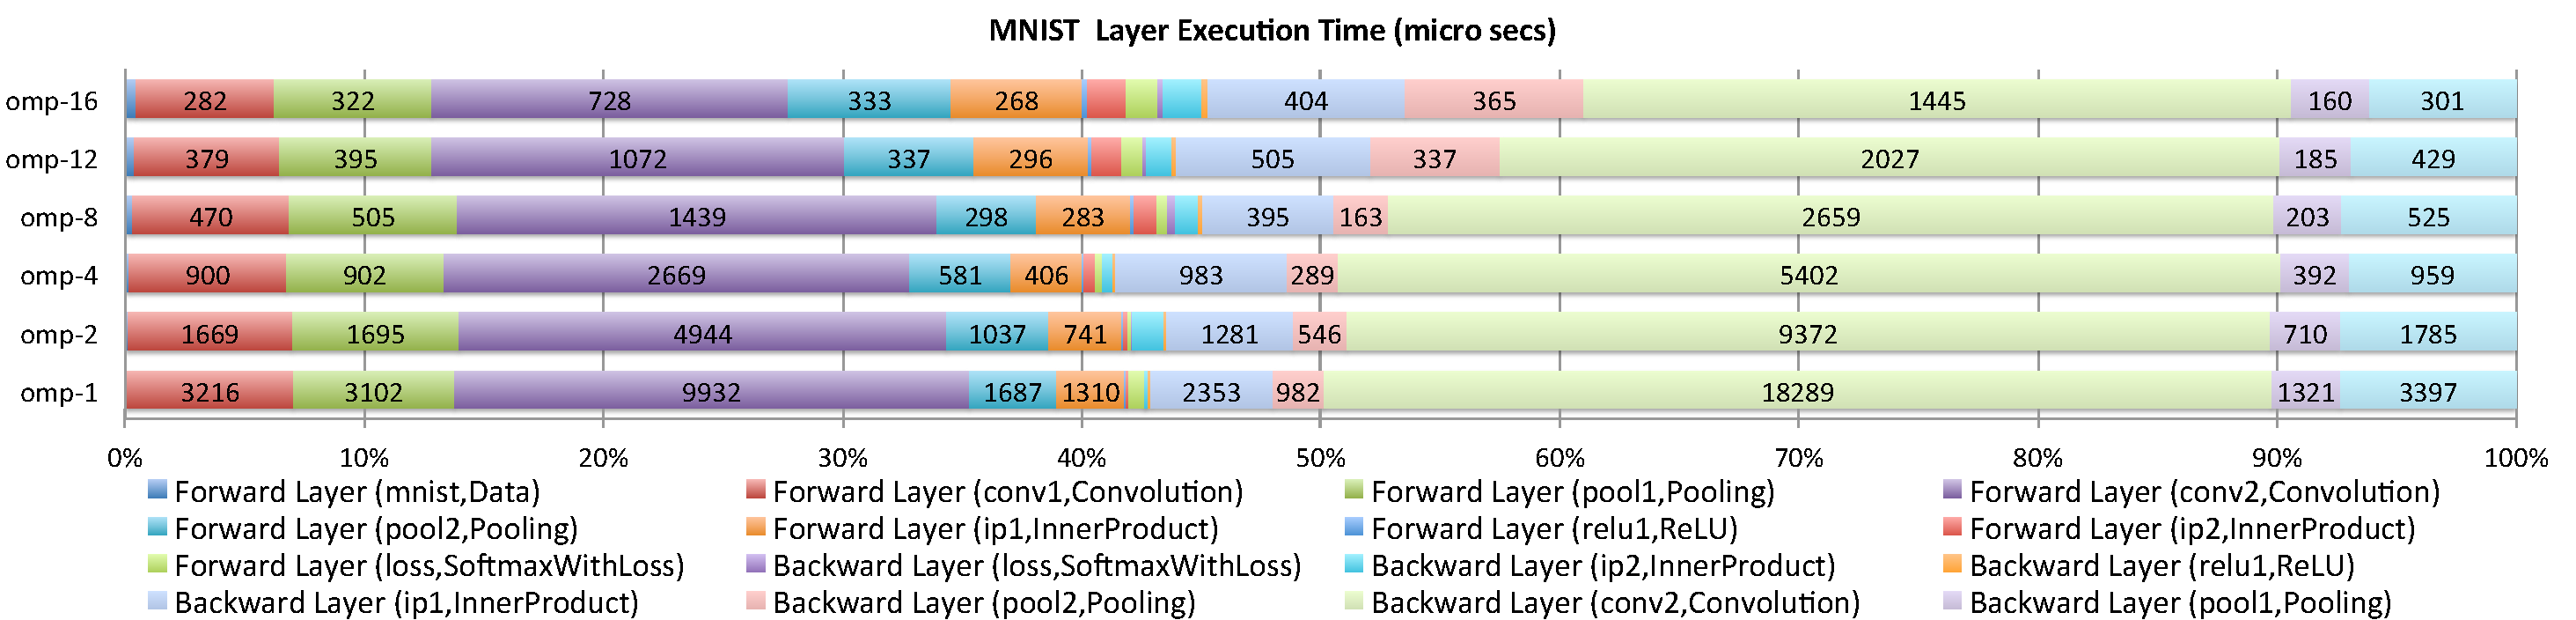
\includegraphics[width=\linewidth]{figures/mnist-rel-abs-time.pdf}
\caption{MNIST - Relative and absolute execution layer time for CPU executions. Layers in the legend are ordered from left-to-right in each horizontal bar. Horizontal bars correspond to the cases of 1, 2, 4, 8, 12 and 16 threads. All execution times are in microseconds.}
\label{fig-mnist-abs-rel}
\end{figure*}

\begin{figure*}[]
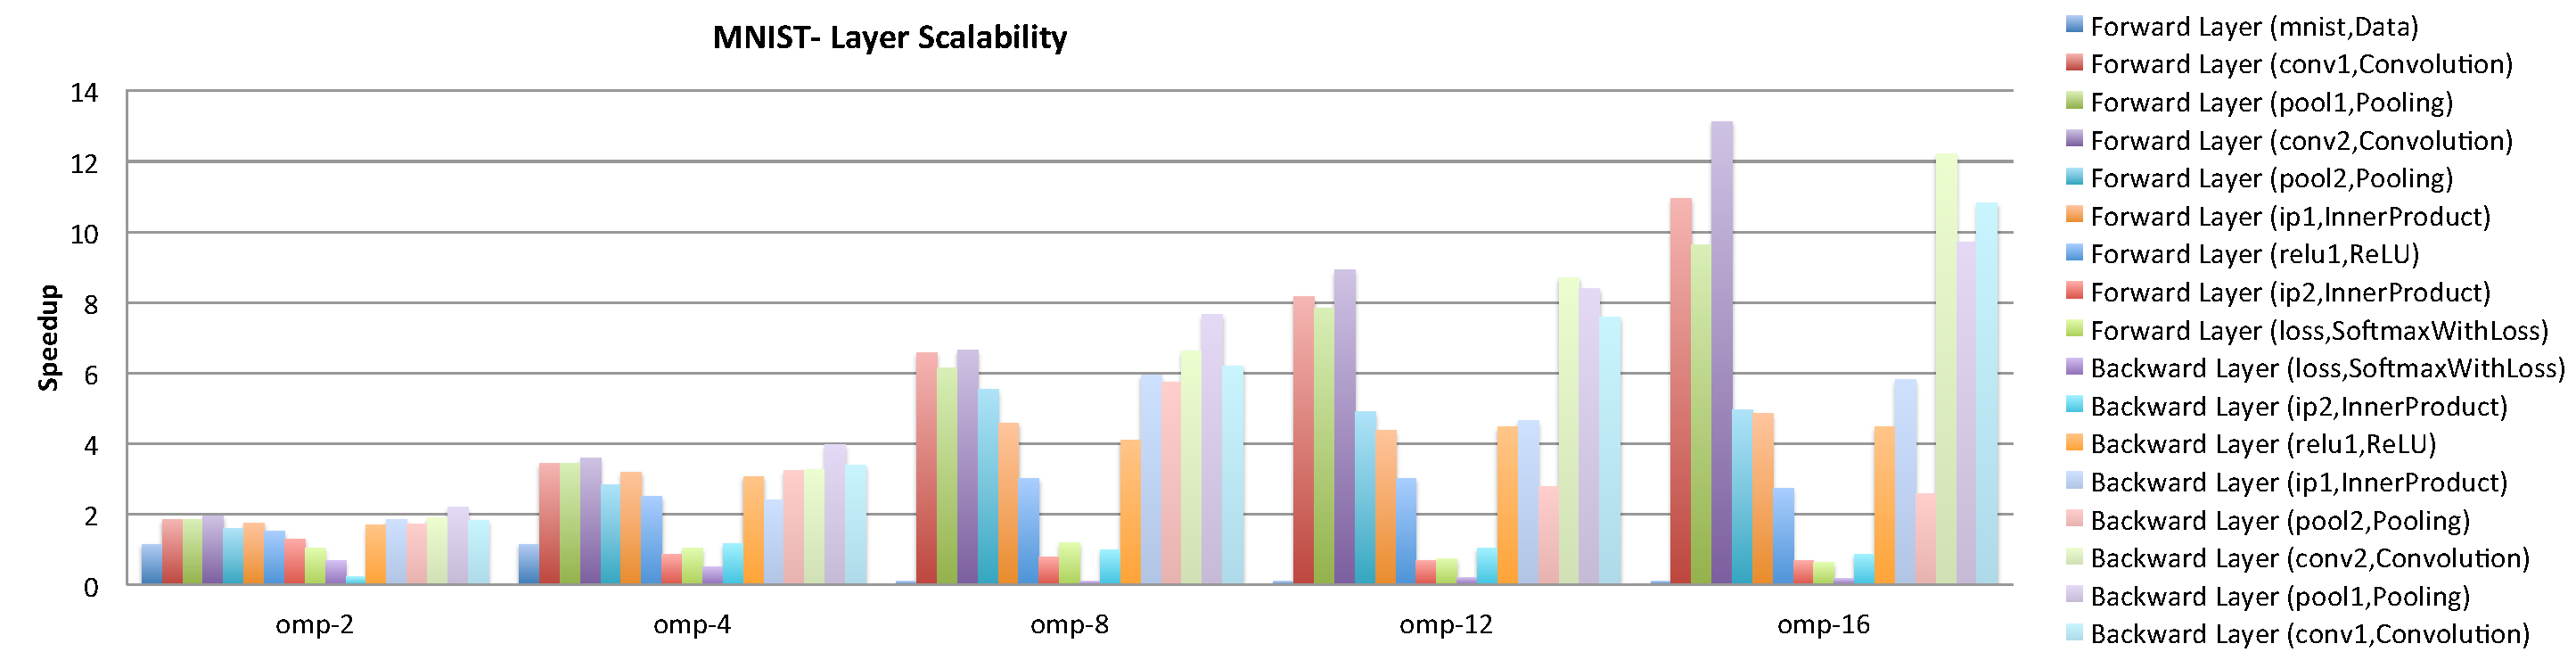
\includegraphics[width=\textwidth]{figures/mnist-scalability-layer.pdf}
\caption{MNIST - Layer scalability for the CPU executions. Layers are identified as in the legend for Figure \ref{fig-mnist-abs-rel}. Layers in the legend are ordered from left-to-right in each cluster. Clusters correspond to the cases of 2, 4, 8, 12 and 16 threads. Y-axis measures speedup factors from the serial CPU execution.}
\label{fig-mnist-scalability}
\end{figure*}

\subsection{MNIST dataset}
For the performance analysis of the MNIST dataset we have first 
developed a per-layer study both coarse-grain and fine-grain parallelizations.For the coarse-grain case we identify what are the main limiting 
performance factors. Then we describe the overall performance of the 
coarse-grain parallelization. 

\subsubsection{Coarse-grain Layer Performance}
Figure \ref{fig-mnist-abs-rel} shows the absolute execution time per layer 
and the relative weight in the overall execution time. Horizontal bars 
correspond to executions with 1, 2, 4, 8, 12 and 16 threads. In general, 
two layers dominate the whole execution: the convolutional and pooling 
layers. No matter the number of threads, these two type of layers always 
account for almost 80\% of total execution time, adding their forward 
and backward passes. Notice that there are different instances of the 
same type of layer but with very different absolute execution time. 
For instance, the \emph{conv1} and conv2 layers, and in a smaller magnitude 
the pool1 and pool2 layers. After the convolutional and pooling layers, 
the next significant layer is the inner product ip1. The rest of layers, 
expose a very small contribution to the overall execution time 
(e.g.: loss, ReLU and ip2 layers in their forward and backward passes).
In general, notice that in each horizontal bar there is a zone where the 
work in each layer phase decreases. This corresponds to the center part, 
composed of the forward and backward passes of pool2, ip1, ReLU, ip2 and loss.
This behavior is associated to the dimensionality reduction that neural 
networks do, and affects the work granularity for the parallelization process.
Moreover, this behavior limits the overall scalability of the training process.

Figure \ref{fig-mnist-scalability} shows the scalability curve of each layer. 
We identify three layer behaviors. First, notice the u-shape of the 
scalability trends for any number of threads. The center points 
correspond to the layers that we have previously identified as not 
significant in the overall execution time (e.g.: loss, ReLU and ip2 layers). 
These layers do not scale at all, but they do not represent a limitation for 
the overall performance. The two sides on the center values correspond 
to the forward and backward passes of the rest layers. For these, we detect 
two types of layer behavior. 

Layers ip1 and pool2 present very poor scalability curves. 
For ip1, in both the forward and backward passes, the layer 
presents speedups of 4,58 and 5,93 for the forward and backward 
pass respectively and with 8 threads. The layer does not improve 
the speedup with more threads. The pool2 layer exposes the same 
behavior with maximum speedup of 5.52 and 5.73 with 8 threads in 
the forward and backward pass respectively. The reason for this 
behavior is two fold. First, notice the two layers are immediately 
stacked one on top of the other. This means that the 
output of the pool2 layer is the input for the ip1 layer. It happens 
that the blob shapes between the two layers do not match. The pool2 
layer is parallelized according to its input blob dimensions, and 
produces its output blob (input blob for ip1) following the resulting 
work and data distribution coming out from the parallelization. When 
it comes the execution of the ip1 layer, its parallelization is done 
according to its input blob dimensions (output blob of pool2), which do 
not match those of the input blob for the pool2 layer. Thus, theres is 
an unavoidable lost of locality for the execution of the ip1 layer. 
Second, both layers suffer from a poor granularity when executing with 
more than 8 threads. In Figure \ref{fig-mnist-abs-rel} we observe that 
with more than 8 threads the forward and backward passes of the two layers 
are in the range of 350 microseconds.

Layers conv1, pool1 and conv2 present good scalability curves. They 
correspond to the layers in both sides of the center part of the 
scalability layer curves. In general, these layers respond well to the 
increments on the number of threads. This is explained by two factors. 
First, all these layers expose a considerable amount of work, as it has 
been indicated with Figure \ref{fig-mnist-abs-rel}. Second, all of them 
are stacked one next to each other within the network, and all of them 
match their input/output blob dimensions. Thus, data locality is 
preserved along the their execution in both the forward and backward passes.
We have detected that although being exactly the same layer, the conv1 
and conv2 layers have close to a 10\% difference in speedup. 
In particular, the conv2 layer exposes greater speedups than conv1. 
This happens more noticeably with more than 8 threads and for the 
forward pass. The difference between the two layers is the position 
they occupy in the layer stack. Conv1 is the immediate layer after the 
data layer in the MNIST network. The data layer is responsible for
feeding the network with data samples. The layer executes sequentially, 
so the data associated to all images generates a memory footprint that is 
not matching the one generated along the parallel execution of the 
conv1 layer. Therefore, the conv1 layer suffers from a poor data 
locality with its immediate previous layer.

%\begin{figure}[]
%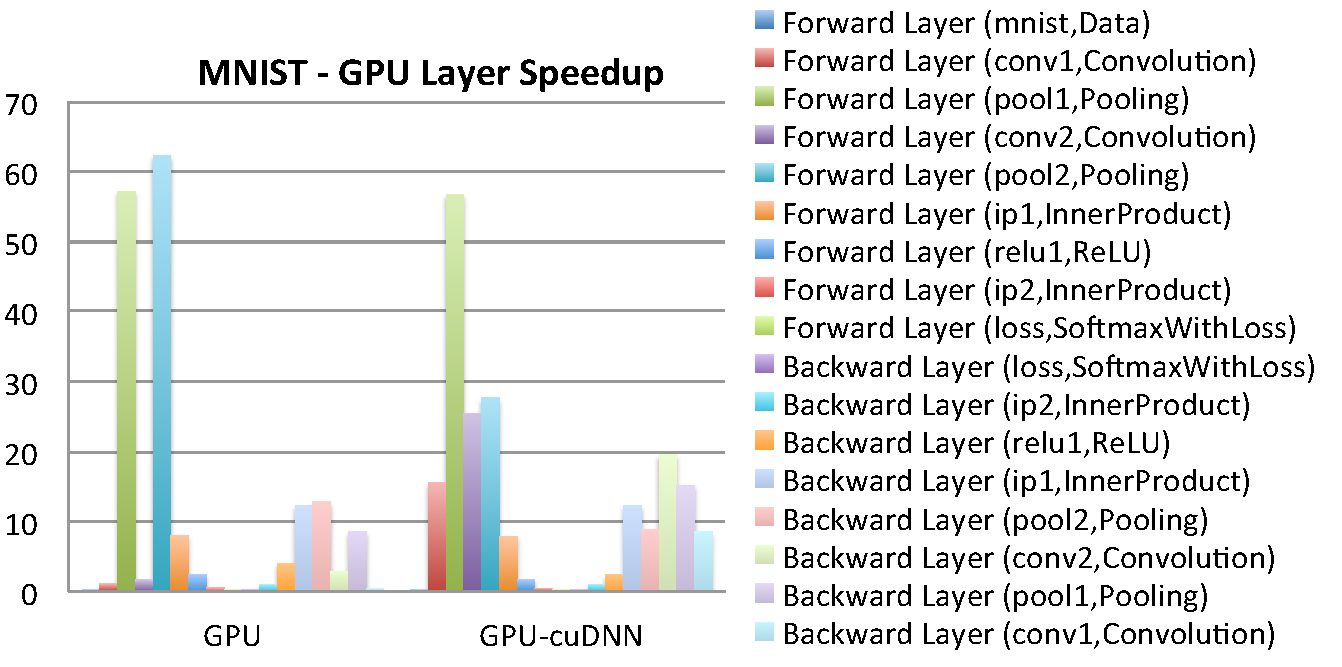
\includegraphics[width=\linewidth]{figures/mnist-gpu-layer-speedup.pdf}
%\caption{\todo{CAPTION}}
%\end{figure}

\begin{figure*}[]
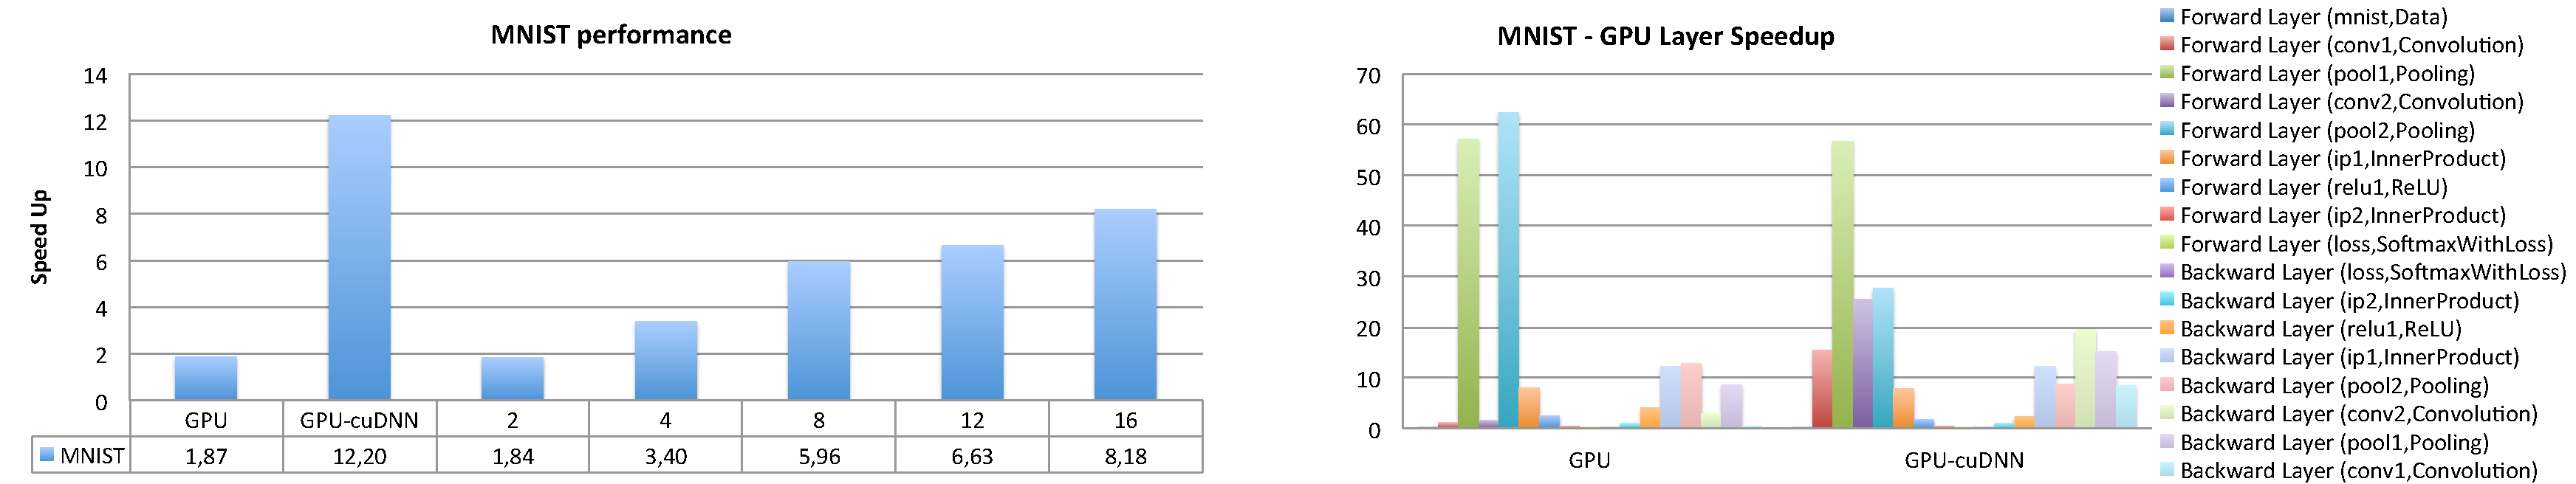
\includegraphics[width=\textwidth]{figures/mnist-abs-perf+gpu-layer.pdf}
\caption{MNIST - \textbf{Leftmost side}: Absolute speedup factors for OpenMP (2, 4, 8, 12 and 16 threads), plain-GPU and cuDNN-GPU versions. performance. \textbf{Rightmost} side: GPU layer scalability for plain-GPU and cuDNN-GPU versions. Layers are identified as in the legend for Figure \ref{fig-mnist-abs-rel}.}
\label{fig-mnist-overall}
\end{figure*}

\subsubsection{Fine-grain Layer Performance}
The fine-grain layer parallelization is available in Caffe in two versions. 
All available layers come with a native GPU implementation of their 
forward and backward pass. We identify this version as the \emph{plain-GPU} 
version. Specifically for the convolutional and pooling layers, Caffe 
includes a cuDNN-based version. We identify this version as the 
\emph{cuDNN-GPU} version. 
%Both present similar execution time distribution 
%as the omp-1 serie in Figure \ref{fig-mnist-abs-rel}: convolutional and 
%pooling layers dominate the GPU execution. 
Rightmost side of Figure \ref{fig-mnist-overall} shows the per-layer 
speedup numbers for the plain-GPU and cuDNN-GPU versions. 
For the plain-GPU version, all layers present speedup below 
the 10$\times$ bar unless for specific exceptions. The pool1 and pool2 
layers expose extraordinary speedups of 57$\times$ and 62$\times$ for their 
forward passes respectively. The pool2 layer presents a speedup of 
12.81$\times$ in its backward pass and the ip1 layer is also above the 
10$\times$ bar with a speedup of 12.25$\times$ in its backward pass.
In contrast, the convolutional layers present a very poor speedup, with 
1.11, 1.63 for the forward passes of conv1 and conv2, and 0.43$\times$ and 2.86$\times$ 
in their respective backward passes. 

For the cuDNN-GPU, the results are similar, unless for the convolutional 
and pooling layers. The conv1 and conv2 layers experiment an extraordinary 
improvement reaching speedups of 15$\times$, 25$\times$, 19$\times$ and 8$\times$ in their 
forward and backward passes. In contrast, the pool2 layer experiments a 
dramatic loss of performance: it drops from 62$\times$ to 27$\times$ in its forward 
pass and from 12.81$\times$ to 8.81$\times$ in its backward pass. More moderately, 
the ReLU layer also suffers a performance drop from 2.47$\times$ to 1.74$\times$ and 
from 4$\times$ to 2,41$\times$ in its froward and backward passes respectively. 
In general, cuDNN corresponds to a case where the industry has deployed 
a highly optimized implementation of layer transformations that well 
understood and no longer in a research stage. In this situation, the 
fine-grain parallelism makes a difference, after the corresponding recoding 
efforts.

%\begin{figure}[b]
%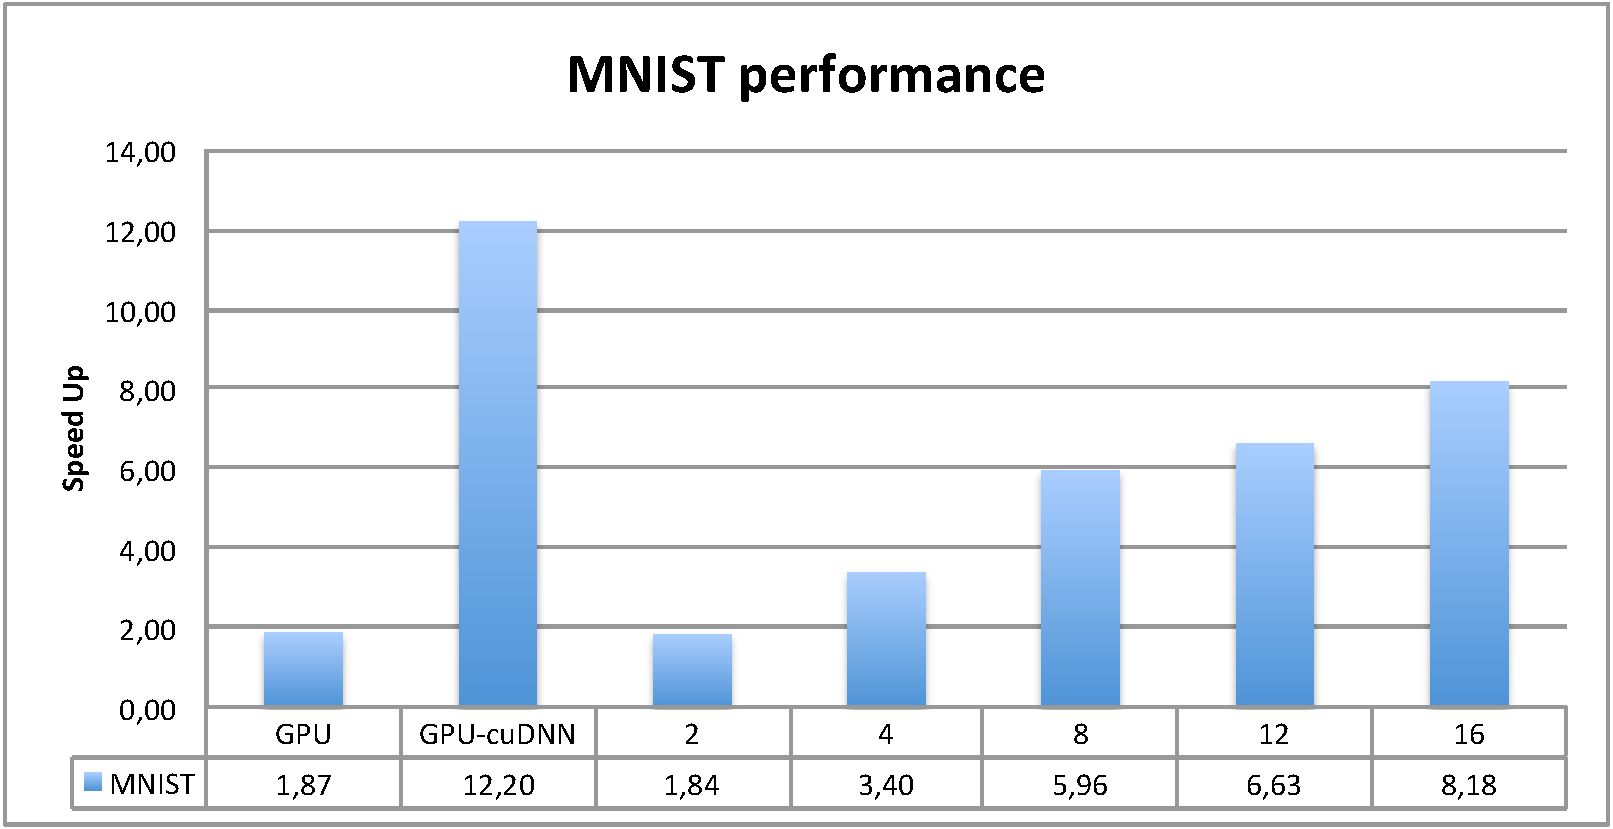
\includegraphics[width=\linewidth]{figures/mnist-abs-perf-all.pdf}
%\caption{\todo{CAPTION}}
%\end{figure}

\subsubsection{Overall Performance}
Figure \ref{fig-mnist-overall} shows the overall performance of
the coarse-grain parallelization and the fine-grain parallelization in 
its two versions GPU and GPU-cuDNN. The coarse-grain reaches a speedup 
close to a 6$\times$ with 8 threads, and 8$\times$ with 16 threads. The lack of 
the scalability for the CPU version is related to the poor scalability 
of fine-grained layers that when executing with 16 threads drag down 
the performance. In addition, we suspect the serial initialization of 
the network structures is giving a suboptimal memory allocation in 
the NUMA nodes. All of this is affecting the final scalability of 
the coarse-grain version. The fine-grain GPU version shows a 
modest speed up close to 2$\times$. The reason for this difference is related 
to the performance of the convolutional layers. In general, this version 
corresponds to a base line defined by the Caffe native implementation 
of the GPU acceleration. It represents a case for the performance the DNN 
community can obtain with a fine-grain parallelization and very significant 
coding efforts. Remember that within Caffe, all layers have to have 
both a CPU and GPU implementation to guarantee GPU acceleration. 
In conclusion, the coarse-grain approach minimizes the coding efforts 
and delivers better performance levels. Of course, when compared to 
the cuDNN case, the fine-grain approach makes a difference. 
It delivers a 12$\times$ speedup. But solutions like the cuDNN framework are 
only available when the layer types and their implementation have become 
a product and are no longer in a research stage. Thus, they can have a 
highly optimized implementation. For a DNN framework like Caffe, 
which is aimed to give support for research in new network architectures 
with novel layer types, the fine-grain parallelism imposes hard recoding 
efforts. In contrast, the coarse-grain option is much more immediate and 
effective.

\begin{figure*}[]
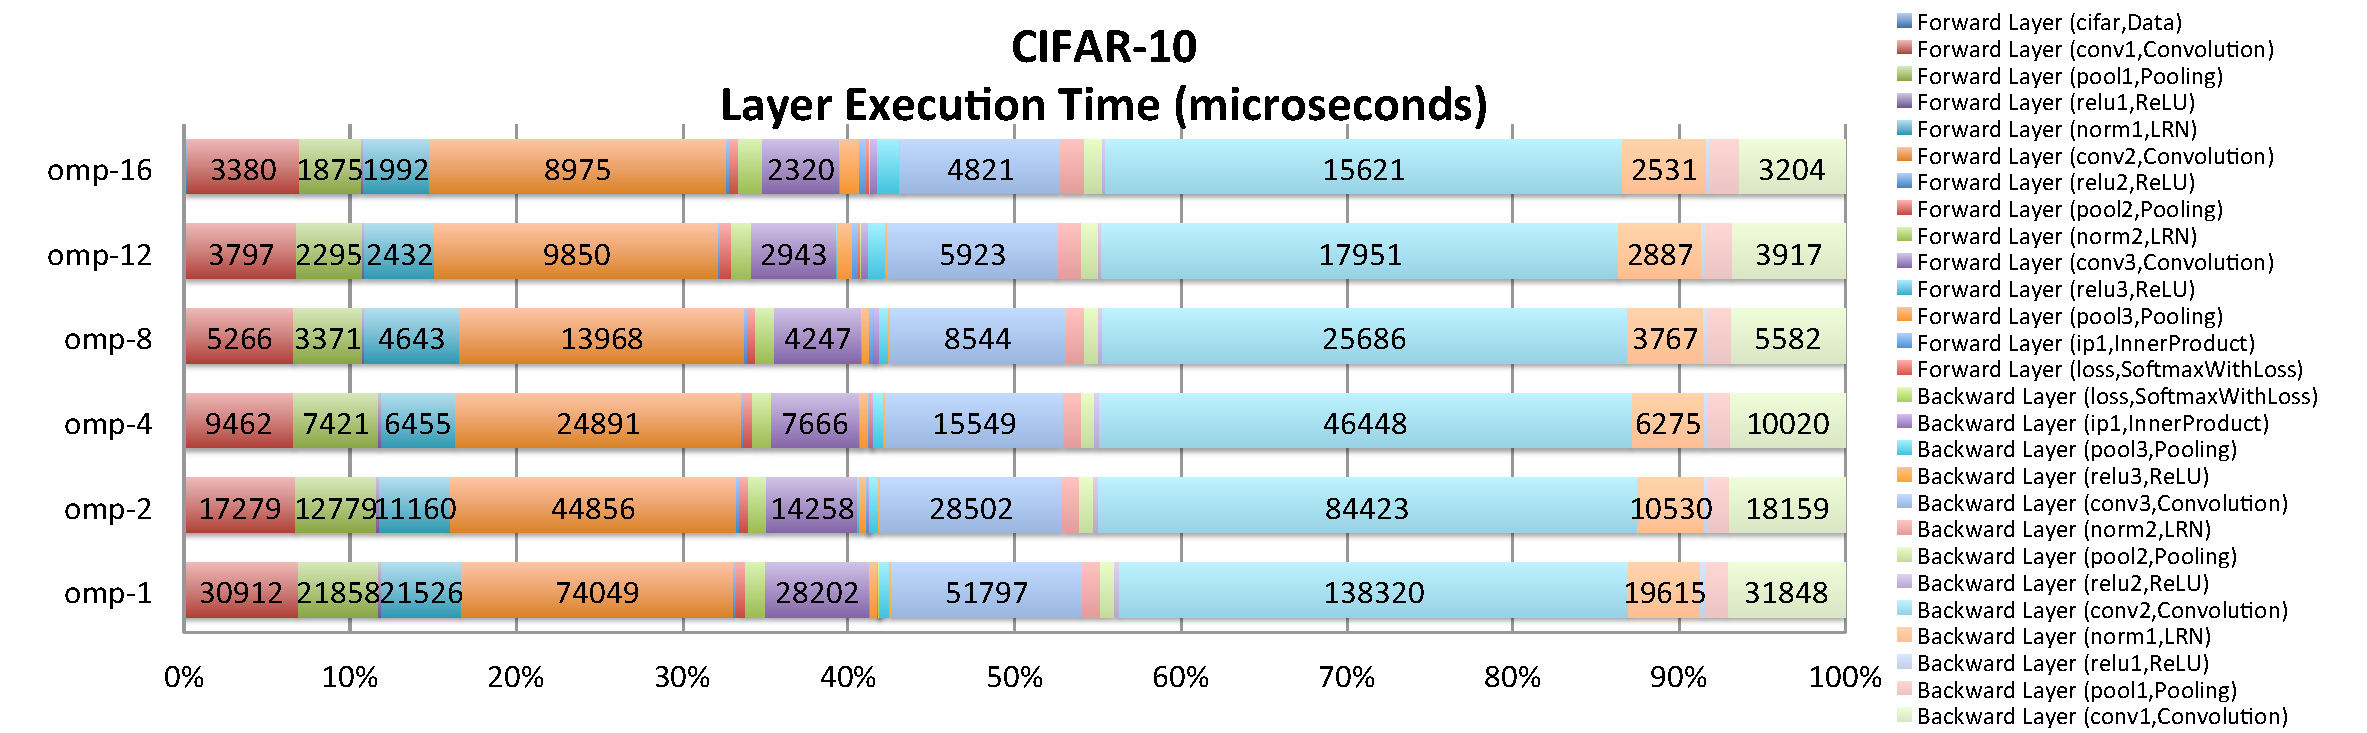
\includegraphics[width=\textwidth]{figures/cifar-abs-rel-time.pdf}
\caption{CIFAR-10 - Relative and absolute execution layer time for CPU executions. Layers in the legend are ordered from left-to-right in each horizontal bar. Horizontal bars correspond to the cases of 1, 2, 4, 8, 12 and 16 threads. All execution times are in microseconds.}
\label{fig-cifar-abs-rel}
\end{figure*}

\begin{figure*}[]
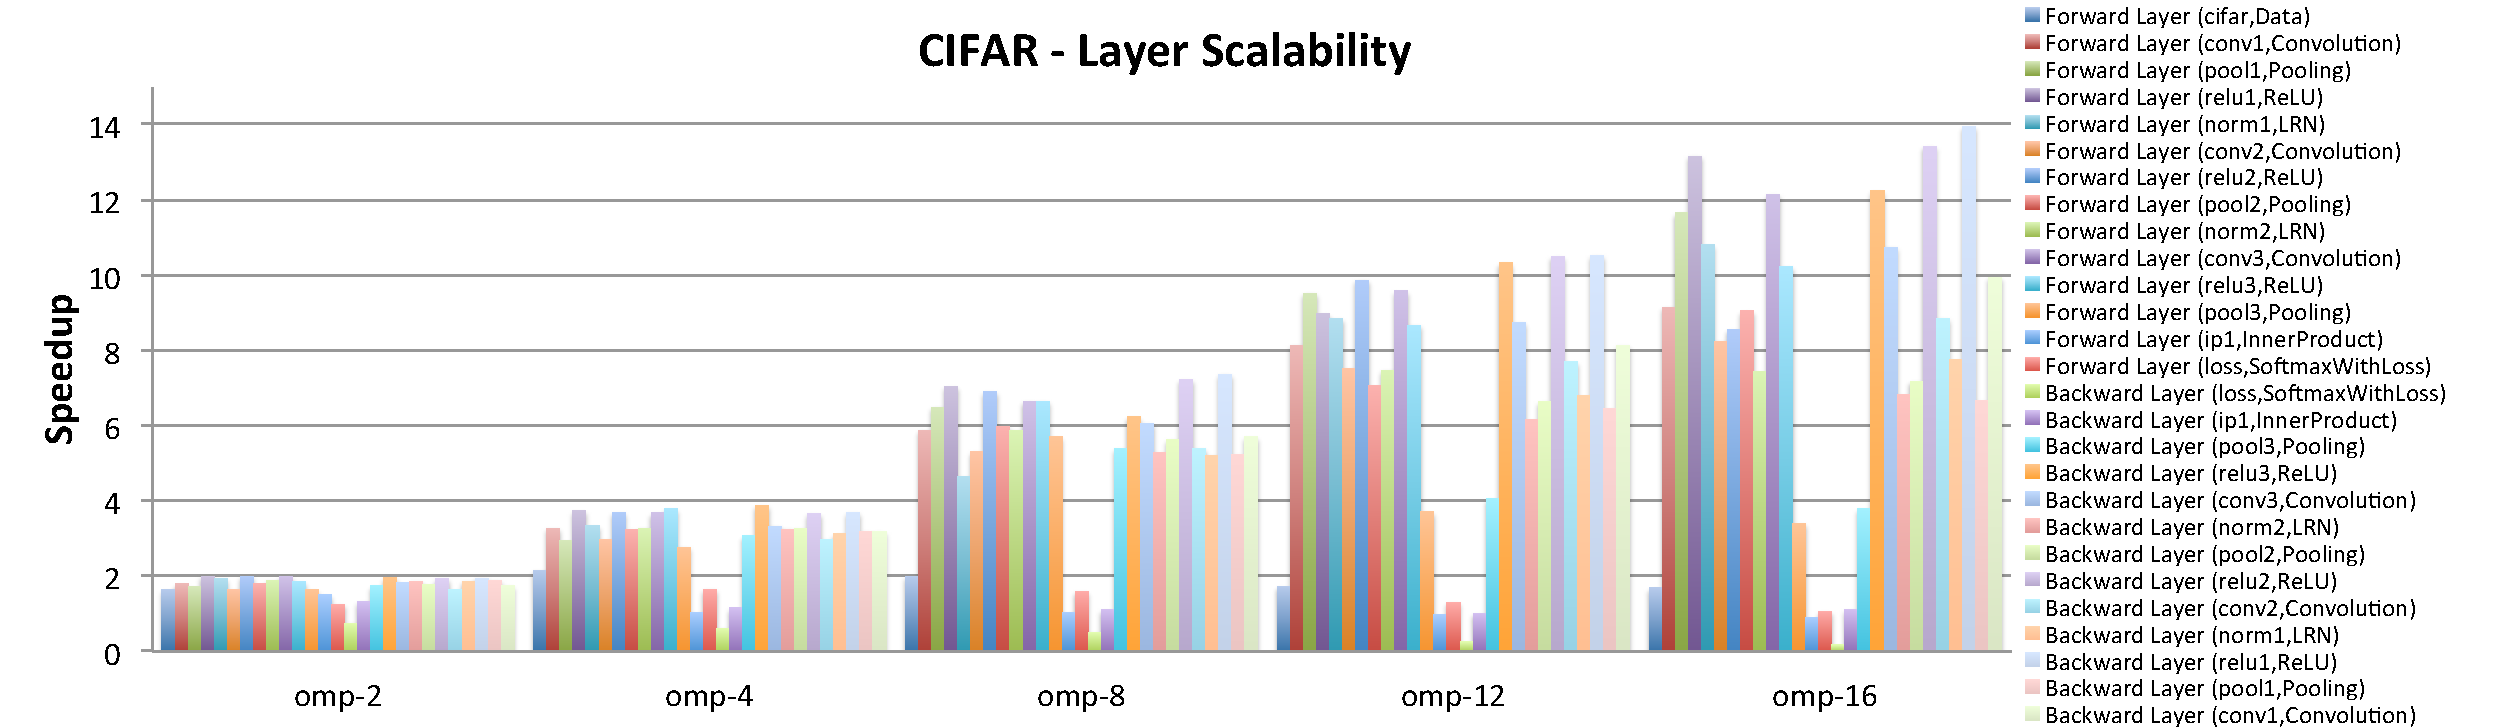
\includegraphics[width=\textwidth]{figures/cifar-scalability-layer.pdf}
\caption{CIFAR-10 - Layer scalability for CPU executions. Layers are identified as in the legend for Figure \ref{fig-cifar-abs-rel}. Layers in the legend are ordered from left-to-right in each cluster. Clusters correspond to the cases of 2, 4, 8, 12 and 16 threads. Y-axis measures speedup factors from the serial CPU execution.}
\label{fig-cifar-scalability}
\end{figure*}

\subsection{The CIFAR-10 case}
For the performance analysis of the CIFAR-10 dataset we have followed the 
same methodology as for the MNIST case. First, we have developed a 
per-layer study both coarse-grain and fine-grain parallelizations. 
For the coarse-grain case we identify what are the main limiting 
performance factors. Then we describe the overall performance of the 
coarse-grain parallelization. 

\subsubsection{Coarse-grain Layer Performance}
The CIFAR-10 dataset generates a work granularity greater than 
the MNIST case. This can be observed in Figure \ref{fig-cifar-abs-rel}. 
The figure shows per-layer absolute execution time and the relative 
weight in the overall execution time. It is clear that just a few 
layers dominate the execution, no matter the number of threads. 
These layers are the convolutional and pooling layers, and with 
less weight the local response normalization layers. In general, 
these layers account for almost 85\% of total execution time in 
all thread configurations. Therefore, the layers with very small 
granularity and exposing very poor scalability curves will not 
determine the overall performance. Only the scalability of these 
dominating layers will determine the effectiveness of the 
parallelization.

Figure \ref{fig-cifar-scalability} shows the scalability curves of all layers. 
Notice the appearance of the u-shape form as long as the number of threads 
increases. The center part of each cluster corresponds to layers of very 
small granularity which do not affect the overall performance. These layers 
are the pool3, ip1 and loss. The center part includes both the forward 
and backward pass of these layers. Leftmost part of each cluster 
correspond to the layer forward pass, the rightmost part corresponds 
to the layer backward pass.

The CIFAR-10 network is organized in three levels all of them with a 
similar organization. First level corresponds to a sequence of a data 
layer plus conv1+pool1+ReLU1+norm1. During the forward pass, the data 
layer fetches the input data (e.g: the batch images) sequentially so 
the conv1 layer suffers from poor locality respect its input data 
(the same situation observed with the MNIST case). The work distribution 
is constant across the conv1, pool1 and ReLU1 layers, and then changes 
for the norm1. According to this, the conv1 has a 
reasonable speedup up to 8 threads (5.87$\times$) but for 16 threads the 
scalability drops with a 9$\times$ speedup. This is explained by the 
sequential execution of its immediate previous layer and by the fact 
that when crossing the 8 thread border, NUMA considerations come into 
play. The effects of data movement are much more visible than when 
just executing in one NUMA node. After the conv1 forward execution, 
the pool1 and ReLU1 layers keep the same work distribution and expose 
reasonable speedups: 6.5$\times$ and 7$\times$ respectively with 8 threads. These 
layers scale up to 11$\times$ and 13$\times$ with 16 threads. The norm1 layer exposes 
a different trend. This layer executes changing the data-thread 
distribution. With 8 threads reaches a 4.6$\times$ speedup and with 
16 threads 10.8$\times$. Regarding the backward pass of all the layers 
in this first level, the relation between the layers are similar, 
but with less scalability. The maximum speedup for 16 threads are 
10$\times$, 6.6$\times$, 7.75$\times$ for the conv1, pool1, ReLU1 and norm1 layers respectively. 
The reduction operations within the backward pass are negligible, 
given the work size in each layer for the CIFAR-10 case. This happens 
in all the network levels.

The second level in the network is composed of layers conv2, ReLU2 
and norm2. In this level, the sizes of the input/output blobs decrease 
and the work granularity too, but with the exception of layer conv2. 
This working set size reduction affects the overall scalability, 
specially with 16 threads. In this level, the maximum speedups are 
8.25$\times$, 8.5$\times$, 9$\times$ and 7$\times$. In this case, the data-thread relation between the 
layers is constant, unless for the norm2 layer. Specifically for the 
first layer in this level, the conv2 layer, its poor scalability is 
related to its immediate previous layer, the norm1 layer. This layer 
changes the data-thread distribution and the conv2 layer is affected 
by this fact. For the backward pass, the performance trends are similar, 
and again the reduction operations do not reduce the overall layer 
scalability.

Finally, the third level is composed by the conv3, ReLU3 and pool3 
layers. This level follows a similar performance trends as the second 
level, with the same relations between its layers and between the 
immediate layer in the second level.

\begin{figure*}[]
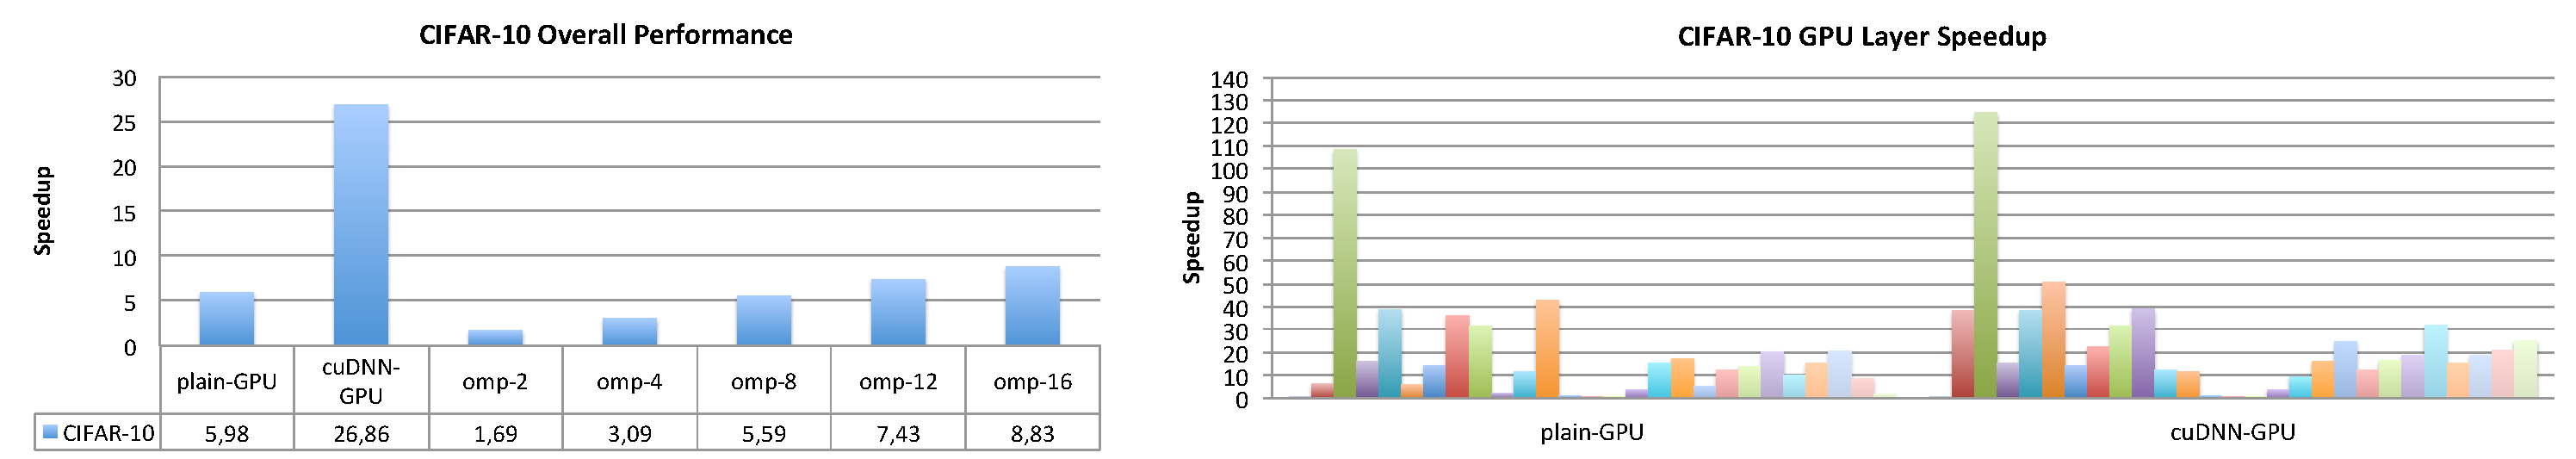
\includegraphics[width=\textwidth]{figures/cifar-abs-perf+gpu-layer.pdf}
\caption{CIFAR-10 - \textbf{Leftmost side}: Absolute speedup factors for OpenMP (2, 4, 8, 12 and 16 threads), plain-GPU and cuDNN-GPU versions. performance. \textbf{Rightmost} side: GPU layer scalability for plain-GPU and cuDNN-GPU versions. Layers are identified as in the legend for Figure \ref{fig-cifar-abs-rel}.}
\label{fig-cifar-overall}
\end{figure*}

\subsubsection{Fine-grain Layer Performance}
Rightmost side of Figure \ref{fig-cifar-overall} shows the per-layer
speedup numbers for the plain-GPU and cuDNN-GPU versions.
For the plain-GPU version, the layer speedups are impressive. 
In the forward pass, all layers present speedups above 10$\times$, and for 
the pooling and LRN layers the speedups are close to 110$\times$ and 40$\times$
respectively (depending on the layer instance and pass in the network). 
The convolutional layers are represent the bottleneck. they present 
speedups between 1.8$\times$ and 6$\times$ depending on the layer position in the 
network and in the pass (forward or backward).

For the cuDNN-GPU, the trends are similar as in the MNISt case 
regarding the convolutional and pooling layers. The convolutional 
layers expose impressive improvements. They switch to performance 
levels close to 50$\times$ of speedup in some cases (conv2 layer).
Some of the pooling layers expose drastic performance drops (pool3 
forward pass switches from 42$\times$ to 11.75$\times$). Others improve the 
performance (pool1 from 8.6$\times$ to 20.9$\times$). 
As it was stated with the MNIST dataset, cuDNN corresponds to a case 
where the industry has deployed a highly optimized implementation of 
specific layer transformations that are well understood and no longer 
in a research stage. In this situation, the fine-grain parallelism makes 
a difference, though after the corresponding recoding efforts.

\subsubsection{Overall Performance}
Figure \ref{fig-cifar-overall} shows the overall performance of
the coarse-grain parallelization and the fine-grain parallelization in
its two versions GPU and GPU-cuDNN. The coarse-grain reaches a speedup
close to a 6$\times$ with 8 threads, and 8.83$\times$ with 16 threads. The lack of
the scalability for the CPU version is related to the poor scalability
of some of the convolutional layers. This is caused by poor data locality caused by consecutive layers with different data-thread patterns. 
In addition, again the serial initialization of
the network structures is giving a suboptimal memory allocation in
the NUMA nodes. All of this is affecting the final scalability of
the coarse-grain version. The fine-grain GPU version shows a
modest speed up close to 6$\times$. Both the fine-grain GPU version and 
coarse-grain CPU version expose problems with the convolutional layers.
In general, the fine-grain GPU version corresponds to the Caffe native 
implementation. This implementation is representative of the 
performance the DNN community can obtain after the associated recoding 
efforts. The coarse-grain parallelization gives similar performance levels, but not requiring the reimplementation of all layers to target the GPU device. 
As with the MNIST case, when compared to the cuDNN case, the fine-grain 
approach makes a difference and this time even greater. cuDNN gives 
extraordinary speedups and it corresponds to an unbeatable implementation 
of the convolutional and pooling layers made by NVIDIA. It delivers a 
27$\times$ speedup. Unfortunately, this performance levels are only available 
for these two layer types. In contrast, the coarse-grain approach is 
immediately available no matter the nature of the deep neural network.

\subsection{Coarse-grain vs Fine-grain: Pros and Cons}
In this section we present the lessons learnt regarding the coarse-grain 
and fine-grain parallelizations of the DNN training process. We identify 
several limiting factors that affect the performance of the 
coarse-grain parallelization. These factors are layer dependent and are 
mainly related to specificities of the layers that determine their 
work distribution, memory footprint, data privatization and ordered 
operations. Also, we identify the advantages and disadvantages of 
the coarse-grain approach in front a fine-grain parallelization. 
The following paragraph describes these limiting factors, 
advantages and disadvantages.

\textbf{Network agnostic}: one important advantage of the coarse-grain 
approach is that it exploits a parallelism level that is independent of 
the nature of the neural network. The batch-level parallelism is 
intrinsic to the gradient descent algorithm. Thus, this approach is 
immediately available and does not require programming efforts to generate 
GPU layer implementations. In addition, the coarse-grain approach 
delivers similar performance levels as the fine-grain approach. 
\textbf{Convergence invariance}: the coarse-grain parallelization does not 
change any training parameters. Thus, the convergence rate is kept 
invariant between the serial and the parallel executions. 
For the DNN community this is an important advantage. Before 
the training, neural networks need a parameter tuning process to ensure 
appropriate convergence. The parallelization has to ensure that the effects of this tuning are kept for the parallel execution.
\textbf{Sequential memory allocation}: the network memory allocation
happens during the network initialization. This process is sequential, 
which causes the layer memory be allocated following a
pattern generated by the initialization code. In terms of performance, 
this pattern is not compatible with those that arise during
the training process.
\textbf{Locality between layers:} the input/output relation across layers
defines a lost of data locality for specific layers. During the forward 
and backward passes, each layer distributes the work according to the 
dimensions of the input blobs. Regarding the data locality, it is 
possible that input and output blobs do not match
their dimensions. Consequently, the work distribution and data-thread
association defined in one layer will not match that one of the
next immediate layer in the stack.
One particular case of this situation corresponds to the data
layers in Caffe. These layers feed the network with input data
organized in batches. Data layers execute in sequentially.
Therefore, a one thread first accesses all data and then the data is
distributed across the cores and the memory hierarchy when the
first parallel processing layer in the network is executes in parallel. 
\textbf{Work unbalance:} coarse grain parallelism is open to work unbalance. 
For the Caffe case, we have detected that batch-level parallelism 
defines very heavy iterations for the parallelized loops.
Therefore, one single loop iteration can cause a high unbalance
between the executing threads. Loop coalescing has been applied to reduce the effect of this problem.
\textbf{Work granularity:} neural networks do
a dimensionality reduction over the processed data.
And this affects the size of the working sets in the network layers.
At some level in the network, the input/output blobs start decreasing their sizes. When this happens, a thread level parallelization
starts suffering from too small work granularity with poor performance levels.
\textbf{Data privatization and reduction operations:} specifically in the
backward pass, the network coefficients are updated per each
sample in the batch. At batch-level, this requires mutual exclusion
mechanisms to guarantee a ordered update. Data privatization has
been needed for this purpose. In terms of performance, given the 
layer granularity, we have not detected these updates top be a 
performance limiting factor.


 

\section{Related Work}
\hyphenation{DistBelief}
This section describes some state of the art deep learning frameworks.
In \cite{JeffDean2012} the authors present a software framework called \emph{DistBelief} that enables model parallelism within a machine (via multithreading) and across machines (via message passing), with the details of parallelism, synchronization and communication managed by
the framework. In addition to supporting model parallelism, the \emph{DistBelief} framework also supports
data parallelism, where multiple replicas of a model are used to optimize a single objective function.

To facilitate training of very large deep networks \emph{DistBelief} supports distributed computation in neural networks and layered graphical models. The user defines the computation that takes place at each node in each layer of the model, and the messages that should be passed during the upward and downward phases of computation.The authors mention in the paper that in certain cases partitioning the model on more than certain number of machines actually slows down training, as communication overhead across hosts starts to dominate in fully-connected layers. One of the main disadvantages of the this framework is that one has to efficiently map the compute blocks onto the host processors such that communication across hosts are minimized to maximally leverage the model parallelism. The coarse level parallelism proposed in this paper is \textbf{network-agnostic} and hence more universally applicable.

In \cite{Coates2013}  presents a deep learning framework with COTS HPC systems: a cluster of GPU servers with Infiniband interconnects and MPI. Their system was able to train 1 billion parameter networks on just 3 machines in a couple of days, and they showed that it can scale to networks with over
11 billion parameters using just 16 machines. While the \emph{DistBelief} framework manages to train a neural network using 16000
CPU cores (in 1000 machines) in just a few days, yet this level of resource is likely well beyond those available to most deep learning researchers.
In this paper the authors present an alternative approach for training large scale networks that leverages inexpensive
computing power in the form of GPUs and introduces the use of high-speed communications infrastructure to tightly coordinate distributed gradient
computations. The authors in this paper makes significant efforts to make the most efficient use of the HPC resources, which may be sometimes well beyond the capabilities of machine learning researchers.

In \cite{Hannun2014} presents a state-of-the-art speech recognition system developed using deep learning.
Their approach uses a well-optimized RNN (recurrent neural network) training system that uses multiple GPUs and use of a novel model partition
scheme to improve parallelization. The authors in this paper develop specific data layout techniques and optimization schemes to scale their training for recurrent networks. The cuDNN \cite{cuDNN} libraries are not general enough and doesn't provide an API for efficiently mapping recurrent computations on the GPU. The coarse grained parallelism proposed in this paper is a simplistic approach that can inherently applied for any feed-forward or recurrent neural network. Hence the proposed parallelism is more universally applicable across diverse application domains.



\section{Conclusions}

\appendix
\section{Appendix Title}


\acks

Acknowledgments, if needed.

% We recommend abbrvnat bibliography style.
\bibliography{ParallelCaffe}{}
\bibliographystyle{abbrvnat}

% The bibliography should be embedded for final submission.

%\begin{thebibliography}{}
%\softraggedright

%\bibitem[Smith et~al.(2009)Smith, Jones]{smith02}
%P. Q. Smith, and X. Y. Jones. ...reference text...
%
%\end{thebibliography}


\end{document}

%                       Revision History
%                       -------- -------
%  Date         Person  Ver.    Change
%  ----         ------  ----    ------

%  2013.06.29   TU      0.1--4  comments on permission/copyright notices

